 %%%%%%%%%%%%%%%%%%%%%%%%%%%%%%%%%%%%%%%%%
% Masters/Doctoral Thesis 
% LaTeX Template
% Version 2.5 (27/8/17)
%
% This template was downloaded from:
% http://www.LaTeXTemplates.com
%
% Version 2.x major modifications by:
% Vel (vel@latextemplates.com)
%
% This template is based on a template by:
% Steve Gunn (http://users.ecs.soton.ac.uk/srg/softwaretools/document/templates/)
% Sunil Patel (http://www.sunilpatel.co.uk/thesis-template/)
%
% Template license:
% CC BY-NC-SA 3.0 (http://creativecommons.org/licenses/by-nc-sa/3.0/)
%
%%%%%%%%%%%%%%%%%%%%%%%%%%%%%%%%%%%%%%%%%

%----------------------------------------------------------------------------------------
%	PACKAGES AND OTHER DOCUMENT CONFIGURATIONS
%----------------------------------------------------------------------------------------

\documentclass[
12pt, % The default document font size, options: 10pt, 11pt, 12pt
oneside, % Two side (alternating margins) for binding by default, uncomment to switch to one side
english, % ngerman for German
doublespacing, % Single line spacing, alternatives: onehalfspacing or doublespacing
%draft, % Uncomment to enable draft mode (no pictures, no links, overfull hboxes indicated)
%nolistspacing, % If the document is onehalfspacing or doublespacing, uncomment this to set spacing in lists to single
%liststotoc, % Uncomment to add the list of figures/tables/etc to the table of contents
%toctotoc, % Uncomment to add the main table of contents to the table of contents
%parskip, % Uncomment to add space between paragraphs
%nohyperref, % Uncomment to not load the hyperref package
headsepline, % Uncomment to get a line under the header
chapterinoneline, % Uncomment to place the chapter title next to the number on one line
%consistentlayout, % Uncomment to change the layout of the declaration, abstract and acknowledgements pages to match the default layout
]{MastersDoctoralThesis} % The class file specifying the document structure

\usepackage[utf8]{inputenc} % Required for inputting international characters
\usepackage[T1]{fontenc} % Output font encoding for international characters
\usepackage{siunitx}
\usepackage{mathpazo} % Use the Palatino font by default
\usepackage[backend=bibtex,style=numeric,natbib=true,autocite=superscript]{biblatex} % Use the bibtex backend with the numeric citation style
\addbibresource{ActiveVision.bib} % The filename of the bibliography
\usepackage[autostyle=true]{csquotes} % Required to generate language-dependent quotes in the bibliography
\usepackage{graphicx}
\usepackage[french, tworuled, figure, linesnumbered]{algorithm2e}

%----------------------------------------------------------------------------------------
%	MARGIN SETTINGS
%----------------------------------------------------------------------------------------

\geometry{
	paper=a4paper, % Change to letterpaper for US letter
	inner= 0.5cm, % Inner margin
	outer=1cm, % Outer margin
	bindingoffset=.5cm, % Binding offset
	top=0.5cm, % Top margin
	bottom=0.5cm, % Bottom margin
	%showframe, % Uncomment to show how the type block is set on the page
}

%----------------------------------------------------------------------------------------
%	THESIS INFORMATION
%----------------------------------------------------------------------------------------

\thesistitle{Optimisation de la vision artificielle bio-inspirée par exploration saccadique de l'environnement} % Your thesis title, this is used in the title and abstract, print it elsewhere with \ttitle
\supervisor{Laurent \textsc{Perrinet}} % Your supervisor's name, this is used in the title page, print it elsewhere with \supname
\examiner{} % Your examiner's name, this is not currently used anywhere in the template, print it elsewhere with \examname
\degree{Master de Neurosciences, spécialité Intégratives et Cognitives} % Your degree name, this is used in the title page and abstract, print it elsewhere with \degreename
\author{Pierre \textsc{Albigès}} % Your name, this is used in the title page and abstract, print it elsewhere with \authorname
\addresses{} % Your address, this is not currently used anywhere in the template, print it elsewhere with \addressname

\subject{Neurosciences computationnelles, Neuromathématiques} % Your subject area, this is not currently used anywhere in the template, print it elsewhere with \subjectname
\keywords{Vision, Biomimétisme, Machine Learning, Computer Vision} % Keywords for your thesis, this is not currently used anywhere in the template, print it elsewhere with \keywordnames
\university{\href{https://www.univ-amu.fr/}{Aix-Marseille Université}} % Your university's name and URL, this is used in the title page and abstract, print it elsewhere with \univname
\department{\href{http://neuro-marseille.org/fr/master-de-neurosciences/}{Master de Neurosciences}} % Your department's name and URL, this is used in the title page and abstract, print it elsewhere with \deptname
\group{\href{http://int.univ-amu.fr/}{Institut de Neurosciences de la Timone}} % Your research group's name and URL, this is used in the title page, print it elsewhere with \groupname
\faculty{\href{https://bio-sciences.univ-amu.fr/}{Faculté des Sciences, département de Biologie}} % Your faculty's name and URL, this is used in the title page and abstract, print it elsewhere with \facname

\AtBeginDocument{
\hypersetup{pdftitle=\ttitle} % Set the PDF's title to your title
\hypersetup{pdfauthor=\authorname} % Set the PDF's author to your name
\hypersetup{pdfkeywords=\keywordnames} % Set the PDF's keywords to your keywords
}

\begin{document}

\frontmatter % Use roman page numbering style (i, ii, iii, iv...) for the pre-content pages

\pagestyle{plain} % Default to the plain heading style until the thesis style is called for the body content

%----------------------------------------------------------------------------------------
%	TITLE PAGE
%----------------------------------------------------------------------------------------

\begin{titlepage}
\begin{center}

{\scshape\LARGE \univname\par}\vspace{1.5cm} % University name
\textsc{\Large Mémoire de Master}\\[0.5cm] % Thesis type

\HRule \\[0.4cm] % Horizontal line
{\huge \bfseries \ttitle\par}\vspace{0.4cm} % Thesis title
\HRule \\[1.5cm] % Horizontal line
 
\begin{minipage}[t]{0.4\textwidth}
\begin{flushleft} \large
\emph{Auteur:}\\
\href{https://github.com/pierrealbiges}{\authorname} % Author name - remove the \href bracket to remove the link
\end{flushleft}
\end{minipage}
\begin{minipage}[t]{0.4\textwidth}
\begin{flushright} \large
\emph{Superviseur:} \\
\href{http://invibe.net/LaurentPerrinet/}{\supname} % Supervisor name - remove the \href bracket to remove the link  
\end{flushright}
\end{minipage}\\[2cm]

\vfill
\large \textit{Un mémoire présenté à\\ \textsc{Ecole Doctorale des Sciences de la Vie et de la Santé}\\en vue de l'obtention du diplôme de\\ \textsc{\degreename}}\\[0.3cm] % University requirement text
\textit{et réalisée au sein de}\\[0.4cm]
\groupname\\[2cm] % Research group name and department name
\small \textit{Durant la période : 12/03/2018 - 08/06/2018}\\[4cm] % Date
%\includegraphics{Logo} % University/department logo - uncomment to place it

\end{center}
\end{titlepage}

%----------------------------------------------------------------------------------------
%	QUOTATION PAGE
%----------------------------------------------------------------------------------------

%\vspace*{0.2\textheight}

%\noindent\enquote{\itshape Wolves have no Kings}\bigbreak

%\hfill Robin Hobb

%----------------------------------------------------------------------------------------
%	ABSTRACT PAGE
%----------------------------------------------------------------------------------------

\renewcommand{\abstractname}{Résumé}
\begin{abstract}
%\addchaptertocentry{\abstractname} % Add the abstract to the table of contents
\end{abstract}

%----------------------------------------------------------------------------------------
%	ACKNOWLEDGEMENTS
%----------------------------------------------------------------------------------------

%\begin{acknowledgements}
%\addchaptertocentry{\acknowledgementname} % Add the acknowledgements to the table of contents
%The acknowledgments and the people to thank go here, don't forget to include your project advisor\ldots
%\end{acknowledgements}

%----------------------------------------------------------------------------------------
%	LIST OF CONTENTS/FIGURES/TABLES PAGES
%----------------------------------------------------------------------------------------

\tableofcontents % Prints the main table of contents

%\listoffigures % Prints the list of figures

%\listoftables % Prints the list of tables

%----------------------------------------------------------------------------------------
%	ABBREVIATIONS
%----------------------------------------------------------------------------------------

%\begin{abbreviations}{ll} % Include a list of abbreviations (a table of two columns)

%\textbf{LAH} & \textbf{L}ist \textbf{A}bbreviations \textbf{H}ere\\
%\textbf{WSF} & \textbf{W}hat (it) \textbf{S}tands \textbf{F}or\\

%\end{abbreviations}

%----------------------------------------------------------------------------------------
%	PHYSICAL CONSTANTS/OTHER DEFINITIONS
%----------------------------------------------------------------------------------------

%\begin{constants}{lr@{${}={}$}l} % The list of physical constants is a three column table

%Speed of Light & $c_{0}$ & \SI{2.99792458e8}{\meter\per\second} (exact)\\
%Constant Name & $Symbol$ & $Constant Value$ with units\\

%\end{constants}

%----------------------------------------------------------------------------------------
%	SYMBOLS
%----------------------------------------------------------------------------------------

%\begin{symbols}{lll} % Include a list of Symbols (a three column table)

%$a$ & distance & \si{\meter} \\
%$P$ & power & \si{\watt} (\si{\joule\per\second}) \\
%Symbol & Name & Unit \\

%\addlinespace % Gap to separate the Roman symbols from the Greek

%$\omega$ & angular frequency & \si{\radian} \\

%\end{symbols}

%----------------------------------------------------------------------------------------
%	THESIS CONTENT - CHAPTERS
%----------------------------------------------------------------------------------------

\mainmatter % Begin numeric (1,2,3...) page numbering

\pagestyle{thesis} % Return the page headers back to the "thesis" style

% Include the chapters of the thesis as separate files from the Chapters folder
% Uncomment the lines as you write the chapters

% Chapter 1

\chapter{Introduction} % Main chapter title
%\addchaptertocentry{Introduction} 
\label{Introduction} % For referencing the chapter elsewhere, use \ref{Chapter1} 

%----------------------------------------------------------------------------------------

% Define some commands to keep the formatting separated from the content 
\newcommand{\keyword}[1]{\textbf{#1}}
\newcommand{\tabhead}[1]{\textbf{#1}}
\newcommand{\code}[1]{\texttt{#1}}
\newcommand{\file}[1]{\texttt{\bfseries#1}}
\newcommand{\option}[1]{\texttt{\itshape#1}}

%----------------------------------------------------------------------------------------

\section{Vision naturelle}
% Rôle de la vision
Tous  les êtres vivants utilisent la vision à un degré ou à un autre, et pour de nombreuses espèces -y compris la notre- elle est même la modalité perceptive principale. Elle est alors primordiale pour appréhender l'environnement et interagir avec celui-ci, que ce soit dans une optique de survie de l'individu ou dans la construction de relations sociales.\\

% Structure générale d'une rétine (cônes/bâtonnets + fovéa/rétine périphérique)
Chez les vertébrés la vision débute à la surface de la rétine, où les cellules photovoltaïques (cônes et bâtonnets) réalisent la transduction des signaux lumineux qui les atteignent en signaux électriques, transmissibles au réseaux nerveux en aval.\\
Les cônes et les bâtonnets sont différenciables par un certain nombre de caractéristiques, notamment leur sensibilité aux longueurs d'ondes lumineuses et leur distribution au sein de la rétine. Ces différences permettent à cette dernière de rester fonctionnelle dans de nombreuses situations, y compris lorsque la luminance est très faible (le seuil absolu de la rétine humaine correspondant à 70 photons) et lui permet donc de nous fournir des informations pertinentes dans une grande variété de contextes.\\
Le champs visuel peut être divisé en deux parties. La vision centrale (environ \SI{2}{\degree} chez l'humain) est soutenue par la fovea, une région rétinienne comprenant uniquement des cônes. On y observe l'acuité visuelle la plus importante (la région présente les champs récépteurs les plus petits de la rétine).\\
La vision périphérique comprends majoritairement des bâtonnets, présente une faible acuité et une perception des couleurs très faible (voir nulle). Elle est par contre très sensible à des variations de luminance et de fréquence spatiale (donc aux mouvements) \autocite{Werner2014}.\\
 L'acuité visuelle diminue en fait avec l'excentricité par rapport à la fovéa. Autrement dit, les champs récepteurs visuels grandissent avec cette excentricité.

% Notion de saccades oculaires/Vision d'une cible en périphérie
Lors de l'exploration de son environnement visuel, un agent va pouvoir détecter des stimuli dans sa vision périphérique mais ne va pas y présenter assez d'acuité pour en réaliser une description précise.
En conséquence, l'agent va réaliser des saccades oculaires (mouvements brefs (20-60\si{\milli\second}) des globes oculaires) afin de placer l'image de la cible (ou tout du moins sa position prédite dans l'espace) au niveau de la fovéa, permettant ainsi de traiter les informations en provenant avec la plus grande précision possible.\\

% Cellules parvo/magno -> rôle de la voie magno
L'activité rétinienne est transmise le long des voies nerveuses visuelles jusqu'au cortex visuel, où sera réalisé la majorité du traitement des informations -notamment haut niveau- qu'elle code. \\
Entre la rétine et le cortex existe un certain nombre d'étapes, mais tout au long de ces voies la distribution rétinienne de l'information (la rétinotopie, figure~\ref{fig:visual_system}) est conservée. 

Dans leurs travaux de 1962 et 1977, Hubel et Wiesel émettent l'hypothèse des courants visuels. Cette hypothèse définit trois voies nerveuses naissant dans le \textbf{corps genouillé latéral} (LGN, où sont présents les corps des types cellulaires donnant leurs noms aux voies) et projetant sur le \textbf{cortex visuel primaire} (V1) :  les voies \textbf{magnocellulaire} (M),  \textbf{parvocellulaire} (P) et  \textbf{koniocellulaire} (K). Chacune de ces voies supporte le transport d'informations codant pour des caractéristiques différentes des stimuli visuels \autocite{Denison2014, Werner2014}.\\
L'activité des cellules M, par exemple, ne distingue pas les couleurs mais est sensible à des différences fines de luminance, de contraste et de fréquence temporelle. Ces caractèristiques semblent lier la voie M notamment au traitement de la luminance et des mouvements \autocite{Denison2014, Werner2014}.

% Voie dorsale, rôle dans la localisation de cible et les saccades oculaires
Cette multiplicité de voies visuelles réalisant des traitements différents des stimuli est conservée au delà de V1, où l'on décrit deux courant sortants : les voies \textbf{ventrale} (transportant et traitant majoritairement pour des informations provenant de la voie P) et la \textbf{dorsale} (transportant et traitant majoritairement pour des informations provenant de la voie M)\autocite{Werner2014, Freeman2011}.\\
La voie ventrale communique ainsi principalement avec les aires cérébrales du lobe temporal, l'activité de son réseau étant primordiale pour la reconnaissance et l'identification des objets visuels. La voie dorsale quant à elle communique principalement avec les aires du lobe pariétal, l'activité de ce réseau étant primordiale pour le traitement des relations spatiales entre les objets visuels ainsi que pour le guidage attentionnel et physique vers eux \autocite{Werner2014, Freeman2011}.\\
Parmi ce réseau dorsal, on trouve l'\textbf{aire intrapariétale latérale} (LIP), qui recoit en partie des informations directement depuis V1 et V2 (contournant donc le traitement d'aires en amont, dont l'aire MT) codant pour des stimuli dans le champs visuel périphérique. Des travaux ont d'ailleurs relié l'activité des neurones du LIP à la plannification des saccades oculaires et à la représentation spatiale des objets visuels.

%----------------------------------------------------------------------------------------

\section{Vision artificielle}
% Motivations\\
La vision représentant notre modalité perceptive principale et les aire dévouées à traiter ses informations occupant une part significative de notre système nerveux central (environ 50\% chez certains primates), l'étudier permet de mieux comprendre le fonctionnement général de notre système nerveux~\autocite{Zhaoping2014}.\\
De nombreux domaines d'étude s'intéressent donc au fonctionnement du système visuel, de ses aspects les plus moléculaires jusqu'aux fonctions les plus intégrées. Parmi eux, les neuromathématiques se basent sur les données expérimentales (anatomique, physiologique et comportementale) pour émettre des modèles mathématiques sur le fonctionnement d'une partie ou de l'ensemble de la modalité visuelle. Idéalement, ces théories doivent pouvoir expliquer son activité dans l'ensemble des contextes observables, mais aussi pouvoir prédire son comportement dans de nouveaux contextes\autocite{Zhaoping2014}.\\
Mais ces modèles ne sont pas une finalité en soi dans la compréhension du système. Ils peuvent permettre d'identifier dans les théories de son fonctionnement des défauts ou des zones obscures à notre compréhension et donc diriger les études expérimentales vers ces points\autocite{Zhaoping2014}.\\
L'identification de ces points et la démonstration de ces théories peut passer par le domaine des neurosciences computationnelles, qui va tenter d'appliquer ces modèles mathématiques dans des modélisations du système nerveux. Au delà de la possible validation ou invalidation des modèles, les neurosciences computationnelles permettent de résoudre des problèmes d'ingénierie (puissance de calcul disponible, vitesse de traitement, adaptabilité à l'environnement, \ldots) en s'inspirant des systèmes biologiques, très optimisés, et donc de créer des systèmes artificiels neuromimétiques plus performants et intégrables dans des systèmes embarqués ou des interfaces cerveau-machine.\\

%Valider l'une des théories neurofonctionnelles de la détection de cible visuelle.
Dans cette étude, nous avons tenté de construire un modèle simple de localisation de cible visuelle dans un champs rétinien (le modèle possède une vision centrale où son acuité est maximale et une vision périphérique dont l'acuité diminue avec l'excentricité). Le fonctionnement du modèle fait écho à une vision simplifiée du fonctionnement du système visuel (figure~\ref{fig:visual_system_simple})\autocite{Zhaoping2014}.\\
Le modèle doit être capable de détecter dans sa vision périphérique une cible visuelle aux caractéristiques simples (représentée par un stimulus provenant le base de données MNIST), de prédire précisémment sa position et de réaliser une saccade oculaire afin de la placer dans sa fovea, ce qui lui permet alors de l'identifier avec une certitude élevée.\\
Pour cela plusieurs méthodes (comprenant elles-mêmes plusieurs sous-méthodes) s'offrent à nous. \\
Les \textbf{modèles de saillance} tentent de décrire une image en fonction des régions (ou pixels) qui présentent la plus grande probabilité de fournir des informations pertinentes et donc qui devraient attirer les saccades. Ces modèles permettent donc de créer des histogrammes de probabilité de fixations oculaires mais présentent certaines limites, dont le fait qu'ils ne vont pas tenter de cibler des objets partiellement ou entièrements cachés\autocite{Butko2010}.\\
Les \textbf{modèles de contrôle}, tentent quant à eux de prédire quelles règles le système devra suivre pour répondre au mieux à une tache. A chaque saccade, de nouvelles informations sur l'environnement sont collectées et permettent de changer l'opinion de l'agent sur le monde\autocite{Butko2010}.

% Chapter Template

\chapter{Matériel et méthodes} % Main chapter title
\label{Materiel_methode} % Change X to a consecutive number; for referencing this chapter elsewhere, use \ref{ChapterX}

%----------------------------------------------------------------------------------------

\section{Support physique et numérique} %Spécificités ordinateur/machine virtuelle, python/libraries versions
L'ensemble des modélisations ont été réalisés sur un ordinateur portable hébergeant une machine virtuelle. Leurs caractéristiques sont rassemblées dans le tableau suivant :\\

\resizebox{19cm}{!}{
\begin{tabular}{| p{4cm} || l | l | p{5cm} | l | l |}
\hline
& Identifiant & Système d'explotation & Processeur & Mémoire vive & Carte graphique\\ \hline
Machine physique & ASUS ROG G75VW & Windows 7 64-bit SP1 & Intel Core I7-3610QM 2,30GHz (8CPU) &  
8 GB (DDR3) & NVIDIA GeForce GTX670M\\ \hline
Machine virtuelle (ressources allouées) & VirtualBox v.5.2.6 & Ubuntu 16.04 & 4 CPU, 90\% des ressources & 
5298 Mo & Support GPU non-utilisé\\ \hline
\end{tabular}
}

Les modélisation ont été réalisées à l'aide du language de programmation \href{https://www.python.org/}{Python} (version 3.6.4) renforcé de la librairie \href{https://www.tensorflow.org/}{TensorFlow} (version 1.4) et de l'interface graphique \href{https://jupyter.org/}{Jupyter}.\\
La base de données \href{http://yann.lecun.com/exdb/mnist/}{MNIST} a été utilisée pour l'apprentissage et l'évaluation du modèle. Elle contient 70.000 images de chiffres manuscrits (60.000 pour l'entraînement, 10.000 pour l'évaluation), centrés et dont la taille a été normalisée. Chaque image est accompagnée d'un label décrivant quel chiffre elle contient.

%----------------------------------------------------------------------------------------

\section{Modèle POMDP} %Description du modèle perception-action, schéma explicatif
Le problème de recherche d'information dans un contexte d'exploration de l'environnement visuel peut être formulé comme un \textbf{processus de décision Markovien partiellement observable} (POMDP) \autocite{Butko2010}. \\
Dans un POMDP (figure~\ref{fig:POMDP}), l'agent perçoit partiellement l'\textbf{état de l'environnement} \textit{S} à un temps \textit{t} (dans ce travail, l'environnement visuel) et peut réaliser des \textbf{actions} \textit{A} (ici des saccades oculaires) qui peuvent avoir des conséquences sur l'environnement et sa perception \textit{O} (l'environnement visuel perçut au travers du champs rétinien). L'agent va ainsi construire un \textbf{état de croyance} \textit{B} (ici la position et la catégorie prédites du stimulus) en fonction des observations et des actions réalisées jusqu'ici \autocite{Butko2010}.

Un tel système doit satisfaire la \textbf{propriété de Markov}, qui décrit que la distribution de probabilité des futurs états ne dépends que de l'état précédent et pas de toute la séquence d'états en amont.\\
Ainsi lors de l'évolution du système dans le temps, on considère que l'état suivant de l'environnement est uniquement influencé par son état actuel et l'action (éventuelle) réalisée par l'agent (équation~\ref{eqn:POMDP_sta}) \autocite{Butko2010}. 

\begin{equation}
p(s_{t+1}|s_{1:t},a_{1:t},o_{1:t}) = p(s_{t+1}|s_{t},a_{t})
\label{eqn:POMDP_sta}
\end{equation}

De même, les observations actuelles de l'agent ne dépendent que de l'état actuel de l'environnement et de l'action (éventuelle) qu'il réalise (équation~\ref{eqn:POMDP_obs}) \autocite{Butko2010}.

\begin{equation}
p(o_{t}|s_{1:t},a_{1:t}) = p(o_{t}|s_{t},a_{t})
\label{eqn:POMDP_obs}
\end{equation}

\begin{equation}
B_{t}^i = p(S_{t} = i|A_{1:t},O_{1:t})
\label{eqn:POMDP_bel}
\end{equation}

Nous construisons ainsi un modèle en deux couches. La première, \textit{détecteur}, est entraînée à prédire la position du stimulus dans l'image, perçu au travers du champs rétinien et permet de réaliser une saccade jusqu'aux coordonnées prédites, permettant d'approcher la cible de la vision fovéale. Chaque saccade permet donc d'optimiser la détection du signal.\autocite{Friston2012}\\
La seconde, \textit{classifieur}, est entraînée à prédire la catégorie du stimulus dans l'image, perçu au travers du champs rétinien et permet d'arrêter l'exploration de l'image lorsque sa prédiction présente une certitude assez élevée.

%----------------------------------------------------------------------------------------

\section{Champs rétinien} %Description du modèle logpolar

Avant d'être utilisée par le modèle, l'image provenant de la base MNIST subit un certain nombre de transformations.\\
Chaque image présente originellement des niveaux de gris sur 28x28 pixels. Cette image est placée au hasard (mais de façon normocentrée) sur une image au fond blanc de 128x128 pixels (figure~\ref{fig:mnist_reshape}).\\
A cette image est ensuite appliqué un \textit{filtre Wavelets} ou un \textit{filtre LogPolar}, deux méthodes permettant d'obtenir un champs rétinien, c'est à dire un filtre visuel dont l'acuité est maximale en son centre (simulant la fovea) et diminuant avec l'excentricité (simulant la vision périphérique). Les produits de ces méthodes et leurs théories sous-jacentes seront décrits dans ce document, mais leurs résultats ne peuvent pas être comparés tels quels, leurs architectures n'étant pas au même niveau d'aboutissement (la couche \textit{classifieur} étant par exemple seulement intégré avec la filtre LogPolar pour le moment).\\
!!! Description filtre wavelets!!! \\
Les effets du \textit{filtre Wavelets} sont visibles sur la figure~\ref{fig:wavelet_effect}.\\
!!! Description filtre LogPolar !!!\\
L'une des forces du filtre LogPolar est sa capacité à modéliser la distribution des champs récepteurs rétinien, mais aussi -en modifiant seulement quelques paramètres- celle d'aires corticales visuelles primaires et associatives \autocite{Freeman2011} et peut donc être ré-utilisé dans le cadre d'un modèle visuel multi-couches neuromimétique, notamment pour la modélisation de la voie visuelle ventrale \autocite{Freeman2011}.

%----------------------------------------------------------------------------------------

\section{Apprentissage supervisé} %Formules du modèle mathématiques soutenant la Régression linéaire multivariée
                                                                    %Prétraitements de l'image (whitening, resize et déplacement cible)

Afin d'obtenir un modèle à la fois performant et adaptable, nous l'avons soumis à un apprentissage supervisé sous la forme d'une \textbf{régression linéaire multivariée} optimisée par \textbf{descente de gradient}.\\
Pour cela, nous calculons une hypothèse $h_{\theta}$ (équation~\ref{eqn:Hypo}) sur la répartition des stimuli en multipliant chacune des valeurs \textit{x} de l'entrée à un poids $\theta$ qui lui est spécifique.

\begin{equation}
h_{\theta}(x) = \theta^{T}x + b
\label{eqn:Hypo}
\end{equation}

Ces poids sont ensuite optimisés par descente de gradient (équation~\ref{eqn:Grad_desc}), où ils sont comparés aux labels \textit{y} des entrées pour un nombre d'exemples et d'itérations fixées. Le paramètre d'apprentissage $\alpha$ influence très fortement l'apprentissage et sa valeur doit être adaptée pour éviter un sous- ou un sur-apprentissage (révélant respectivement une valeur trop faible ou trop importante).\\

\begin{equation}
\theta_j := \theta_j - \alpha \frac{1}{m} \sum_{i=1}^m (h_\theta(x^i) - y^i)x_{j}^i
\label{eqn:Grad_desc}
\end{equation}

En parallèle de l'entraînement peut être calculé le coût $J(\theta)$ (équation~\ref{eqn:Cost}), dont l'évolution au cours de l'entraînement est un indicateur de l'efficacité de l'apprentissage. Sa valeur devant décroitre au cours du temps, l'optimisation du modèle peut se faire en tentant de la réduire au maximum.

\begin{equation}
J(\theta) = \frac{1}{2m} \sum_{i=1}^m (h_\theta(x^i)-y^i)^2
\label{eqn:Cost}
\end{equation} 
% Chapter Template

\chapter{Résultats} % Main chapter title
 
\label{Résultats} % Change X to a consecutive number; for referencing this chapter elsewhere, use \ref{ChapterX}

%----------------------------------------------------------------------------------------

\section{Apprentissage supervisé}

L'étape de benchmarking du paramètre d'apprentissage $\alpha$ (équation~\ref{eqn:Grad_desc}) permet de rendre compte de son importance sur l'efficacité de l'apprentissage et du modèle. \\
Dans le cadre du filtre \textit{Wavelets}, on peut ainsi observer qu'une valeur $\alpha\geq0.4$ entraîne un sur-apprentissage très important (le coût augmente fortement au cours de l'entraînement, figures~\ref{fig:benchmark_surApp1} et \ref{fig:benchmark_surApp2}), tandis que $\alpha=0.3$ semble représenter une valeur optimale pour l'apprentissage (figure~\ref{fig:benchmark_alpha}).\\
Dans le cadre du filtre \textit{LogPolar}, deux jeux de poids indépendants doivent être optimisés pendant l'apprentissage,  correspondant respectivement aux couches \textit{détecteur} et \textit{classifieur}. Chaque couche possède ainsi son propre paramètre $\alpha$ ($\alpha_{detect}$ et $\alpha_{classif}$) et l'on peut donc calculer leurs coûts indépendamments (figure~\ref{fig:logpolar_cost}).

%----------------------------------------------------------------------------------------

\section{Prédiction de la position}

Après entraînement, le modèle est capable de détecter la cible dans son environnement et de prédire précisemment sa position (figure~\ref{fig:saccades_wavelets} et \ref{fig:saccades_logpolar}). Il est ensuite capable d'utiliser cette prédiction pour réaliser une saccade aux coordonnées prédites de la cible visuelle, ce qui modifie en conséquence sa perception de l'environnement.\\
Mais une seule saccade n'est pas toujours suffisante pour atteindre la cible (figure~\ref{fig:sacc_nombre}) et le nombre de saccades nécessaires augmente avec la distance initiale de la cible du centre de fixation (figure~\ref{fig:sacc_distance}). Cette relation pourrait provenir de la diminution de l'acuité avec l'excentricité dans la champs visuel (provoquée par le champs rétinien), entraînant une diminution de la précision des prédictions (figure~\ref{fig:err_distance})

%----------------------------------------------------------------------------------------

\section{Prédiction de la catégorie}

%----------------------------------------------------------------------------------------

% Chapter Template

\chapter{Discussion et perspectives} % Main chapter title

\label{Discussion} % For referencing this chapter elsewhere, use \ref{Discussion}

%----------------------------------------------------------------------------------------
Notre modèle semble ainsi capable de s'inspirer du fonctionnement d'un modèle POMDP pour réaliser à tour de rôle une observation de son environnement et une action ayant pour objectif d'améliorer la perception de cet environnement.
L'agent va donc réaliser une série de saccades jusqu'à réussir à placer la cible visuelle au niveau de sa fovéa, où sa description (ici sa catégorisation) pourra être réalisée avec la plus grande accuité possible, et donc avec le plus grand taux de réussite. Ce comportement `'atteindre-et-décrire`' instauré par le fonctionnement séquentiel semble cohérent avec ce que l'on peut observer dans les systèmes biologiques \autocite{Werner2014, Najemnik2005}. \\
En complément à ces observations sur le comportement général du modèle, nous avons pu observer que plus une cible est éloignée de la fovéa de l'agent lorsqu'elle est présentée initialement, moins ses prédictions seront précises et en conséquences plus nombreuses seront les saccades destinées à atteindre la position de la cible. 
Encore une fois, ce comportement semble cohérent avec ce que l'on observe dans les systèmes biologiques. 
A noter toutefois que le profil de performances du modèle, notamment concernant l'évolution de la taille de ses erreurs de prédiction avec l'excentricité de la cible, correspond à de faibles performances biologiques. 
Plus exactement, le modèle semble présenter un profil de performances similaire au système biologique lorsque la cible est présentée peu de temps (150ms), mais lorsqu'elle est présentée plus longtemps (1s) les performances du système biologique ne semblent pas être influencées par l'excentricité de la cible. Des comparaisons quantitatives seront ici nécessaires pour confirmer ou infirmer ces similarités \autocite{Uddin2004}.\\

% Prospects
	% Modèle probabiliste
	% Modif entrainement  utiliser classifieur pour réaliser apprentissage détecteur
	% Bruit écologique
	% Implémentation robotique
	
Plusieurs étapes ont d'ores et déjà été identifiées afin de rendre le modèle à la fois plus performant et plus proche d'une certaine réalité neurologique. \\
La première consistera en la modification de la prédiction du modèle (à l'heure actuelle, la prédiction correspond à deux coordonnées `'certaines`' où la cible devrait être présente) en prédiction probabiliste. 
Cette amélioration permettrait de traiter la perception du modèle comme une carte de probabilité où chaque point de l'espace est relié à une probabilité de contenir la cible. Ainsi la prédiction ne sera pas réalisée sur un point précis de l'espace mais sur une distribution de probabilités dont l'ecart-type devrait augmenter avec l'excentricité (d'après les résultats observés sur la figure~\ref{fig:err_distance}). De plus, cette carte de probabilité se mettant à jour à chaque nouvelle saccade (puisqu'une nouvelle observation de l'environnement est alors réalisée), il devient possible de cumuler les probabilités au cours du temps pour aboutir à un modèle doté d'une mémoire. \autocite{Butko2010, Najemnik2005} \\

Une seconde étape sera de reconsidérer entièrement les méthodes d'apprentissage afin de non seulement augmenter fortement les performances du \textit{classifieur}, pour l'instant loin d'approcher les performances standards des modèles \textit{machine learning} de vision artificielle, mais aussi de tenter d'augmenter au maximum les performances du \textit{détecteur} pour tenter d'atteindre les performances biologiques. \\
L'une des solutions envisageables pour ce dernier point consiste en la transition d'un apprentissage indépendant des deux couches, comme c'est le cas actuellement, vers un modèle d'apprentissage utilisant la sortie (sous la forme d'une carte de probabilité) du \textit{classifieur} pour guider l'entraînement (c'est à dire s'en servir comme d'un label) du \textit{détecteur}. Cette optique permettrait non seulement d'améliorer les performances du modèle, mais aussi d'augmenter son autonomie vis à vis de l'utilisateur humain en produisant lui-même une partie de ses labels d'apprentissage. \\

Lorsque le modèle présentera des performances jugées suffisantes, l'étape suivante sera probablement de le mettre à l'épreuve dans des conditions pour lesquelles il n'aura pas été programmé afin de tester la robustesse de la généralisation obtenue grâce à l'apprentissage automatisé. Pour cela, l'un des moyens à notre disposition est d'altérer la qualité de l'image utilisée en entrée via l'introduction de bruit. 
Idéalement, ce bruit devra être construit pour suivre des règles écologiques, c'est à dire qu'il devra modéliser le bruit que l'on peut retrouver lors d'une perception naturelle de l'environnement visuel. Deux méthodes sont pour le moment envisagées : introduire des pseudo-stimulis créés en `'mélangeant`' des stimuli utilisés pour l'apprentissage (permettant d'obtenir des régions comprenant les mêmes variances de niveaux de gris que lors de la présence d'un stimulus réel mais sans présenter d'information pertinente) et/ou créer un bruit corrélé par transformation mathématiques \autocite{Najemnik2005}. \\

Finalement, lorsque le modèle aura été entraîné, évalué et optimisé dans un ensemble de contextes artificiels, il deviendra envisageable de soumettre son fonctionnement à des contextes écologiques en l'implémentant dans un système autonome.
L'introduction effective du paradigme POMDP permettra à l'agent de choisir l'action la plus adaptée en fonction de sa perception de son environnement et de la tâche à réaliser, tandis la présence de l'apprentissage automatisé et de l'approche neuromimétique (vision rétinienne) permettra de conserver une performance élevée (notamment en adaptabilité et en vitesse de réaction) tout en diminuant au maximum la puissance de calcul et la consommation d'énergie nécessaires à son fonctionnement. \autocite{Potthast2016} \\
En prenant pour example un agent robotisé mobile, tel qu'un drone, dont la tâche serait de reconnaitre un objet ou un visage dans son environnement visuel, ce modèle pourrait lui permettre de choisir de façon active et autonome quelle action choisir (réaliser une saccade et si oui en visant quelle position, réaliser un mouvement et si oui lequel parmi 6 directions et 4 rotations disponibles) suivant son contexte environnemental et les informations qui lui sont accessibles (position estimée de l'agent par rapport à la cible, taux de certitude de l'identification, environnement observé, etc) afin de réaliser sa tâche de façon optimale. \autocite{Potthast2016} \\ 
%\include{Chapters/Chapter5} 

%----------------------------------------------------------------------------------------
%	BIBLIOGRAPHY
%----------------------------------------------------------------------------------------

\printbibliography[heading=bibintoc]

%----------------------------------------------------------------------------------------
%	THESIS CONTENT - APPENDICES
%----------------------------------------------------------------------------------------

\appendix % Cue to tell LaTeX that the following "chapters" are Appendices

% Include the appendices of the thesis as separate files from the Appendices folder
% Uncomment the lines as you write the Appendices

% Appendix A

\chapter{Figures} % Main appendix title

\label{Figures} % For referencing this appendix elsewhere, use \ref{AppendixA}

%%%%% Introduction %%%%%

\begin{figure}[th]
\centering
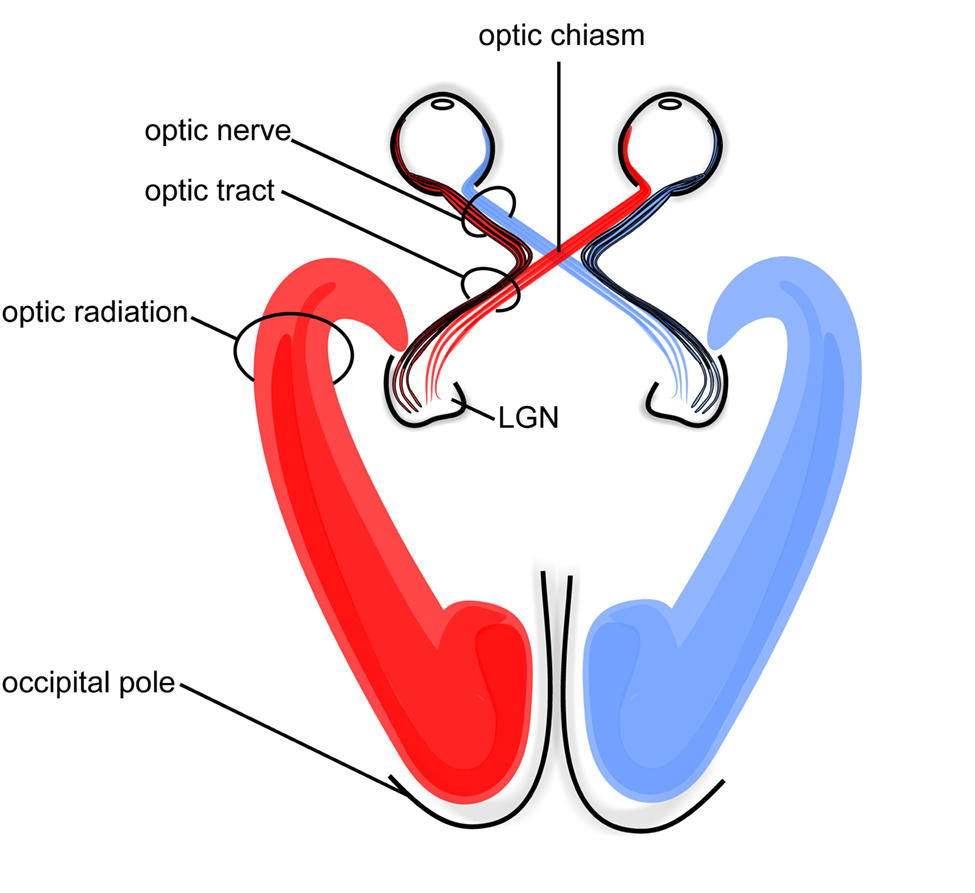
\includegraphics{Figures/visual_system}
\decoRule %puts an aesthetic horizontal line below the image
\caption[Figure]{Schéma des voies visuelles précorticales humaines (adapté de Hofer S. et al., 2010 via Wikimedia Commons [CC BY 3.0])}
\label{fig:visual_system}
\end{figure}

\begin{figure}[th]
\centering
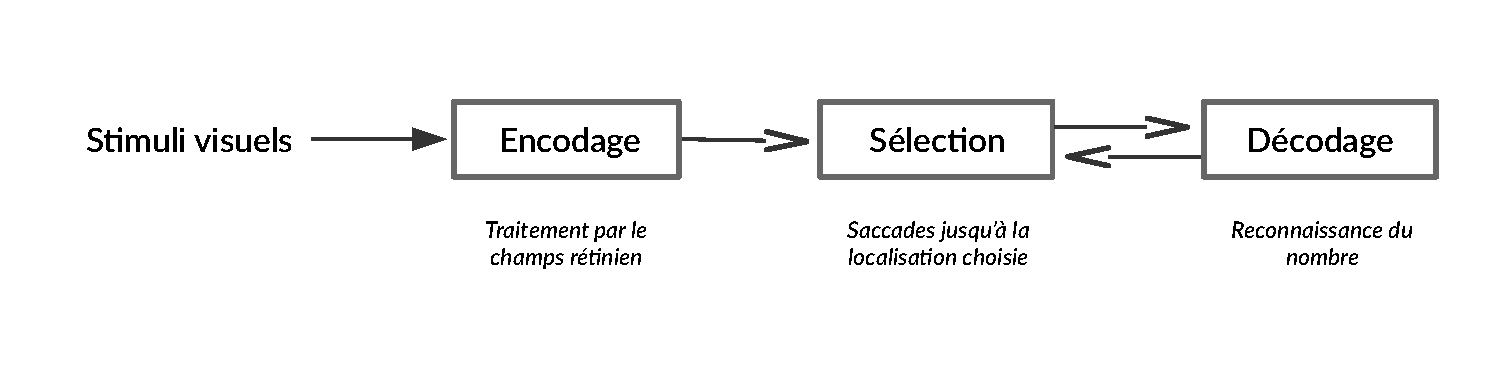
\includegraphics[scale=0.75]{Figures/visual_system_simple}
\decoRule %puts an aesthetic horizontal line below the image
\caption[Figure]{Schéma simplifié du fonctionnement du système visuel avec son \textit{équivalence dans le modèle} (adapté de \cite{Zhaoping2014})}
\label{fig:visual_system_simple}
\end{figure}

%%%%% Matériel et méthodes %%%%%

\begin{table}
\resizebox{19cm}{!}{
\begin{tabular}{| p{4cm} || l | l | p{5cm} | l | l |}
\hline
& Identifiant & Système d'explotation & Processeur & Mémoire vive & Carte graphique\\ \hline
Machine physique & ASUS ROG G75VW & Windows 7 64-bit SP1 & Intel Core I7-3610QM 2,30GHz (8CPU) &  
8 GB (DDR3) & NVIDIA GeForce GTX670M\\ \hline
Machine virtuelle (ressources allouées) & VirtualBox v.5.2.6 & Ubuntu 16.04 & 4 CPU, 90\% des ressources & 
5298 Mo & Support GPU non-utilisé\\ \hline
\end{tabular}
}
\caption[Tableau]{Matériel physique et numérique utilisé pour réaliser les modélisations}
\label{tab:materiel}
\end{table}

\begin{figure}[th]
\centering
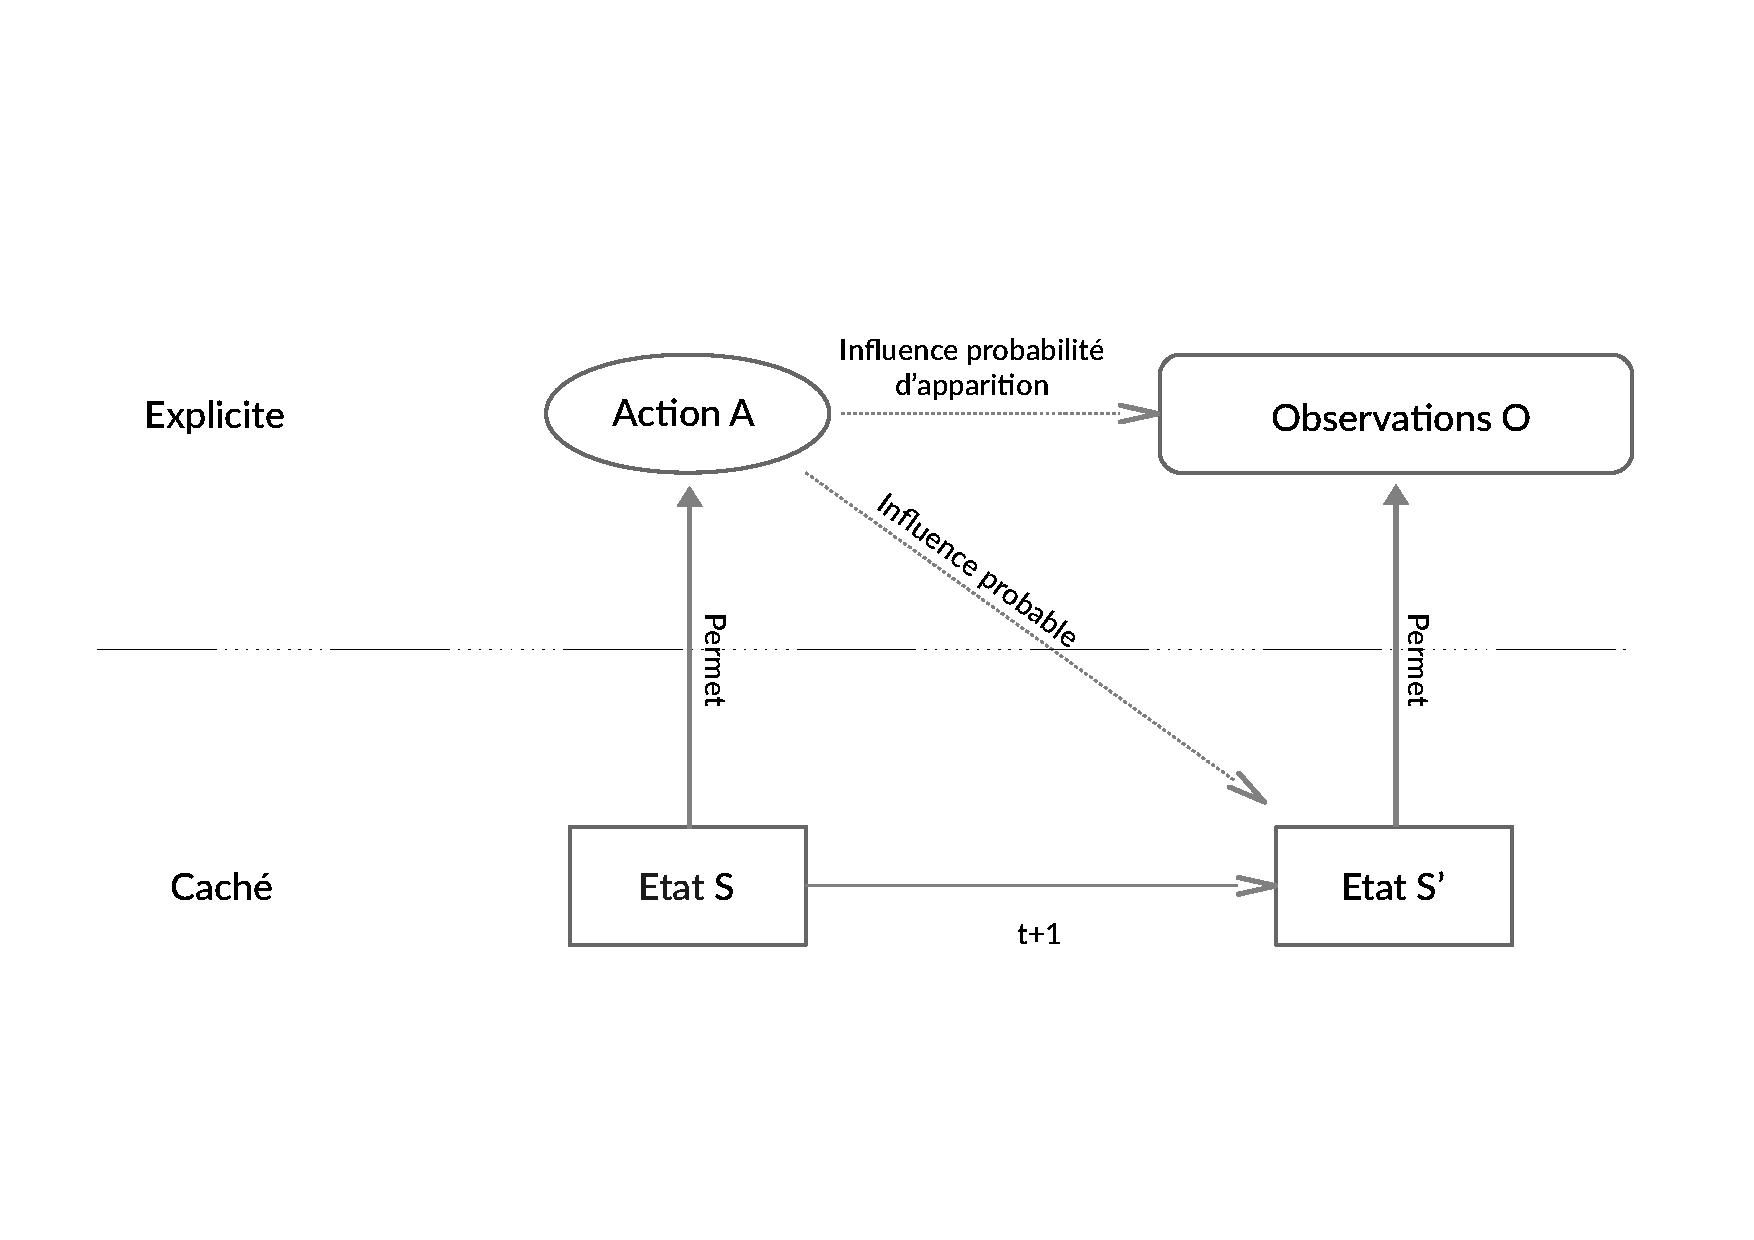
\includegraphics[scale=0.45]{Figures/POMDP}
\decoRule %puts an aesthetic horizontal line below the image
\caption[Figure]{Schéma des interations entre l'agent et son environnement au cours du temps dans un modèle POMDP}
\label{fig:POMDP}
\end{figure}

\begin{figure}[th]
\centering
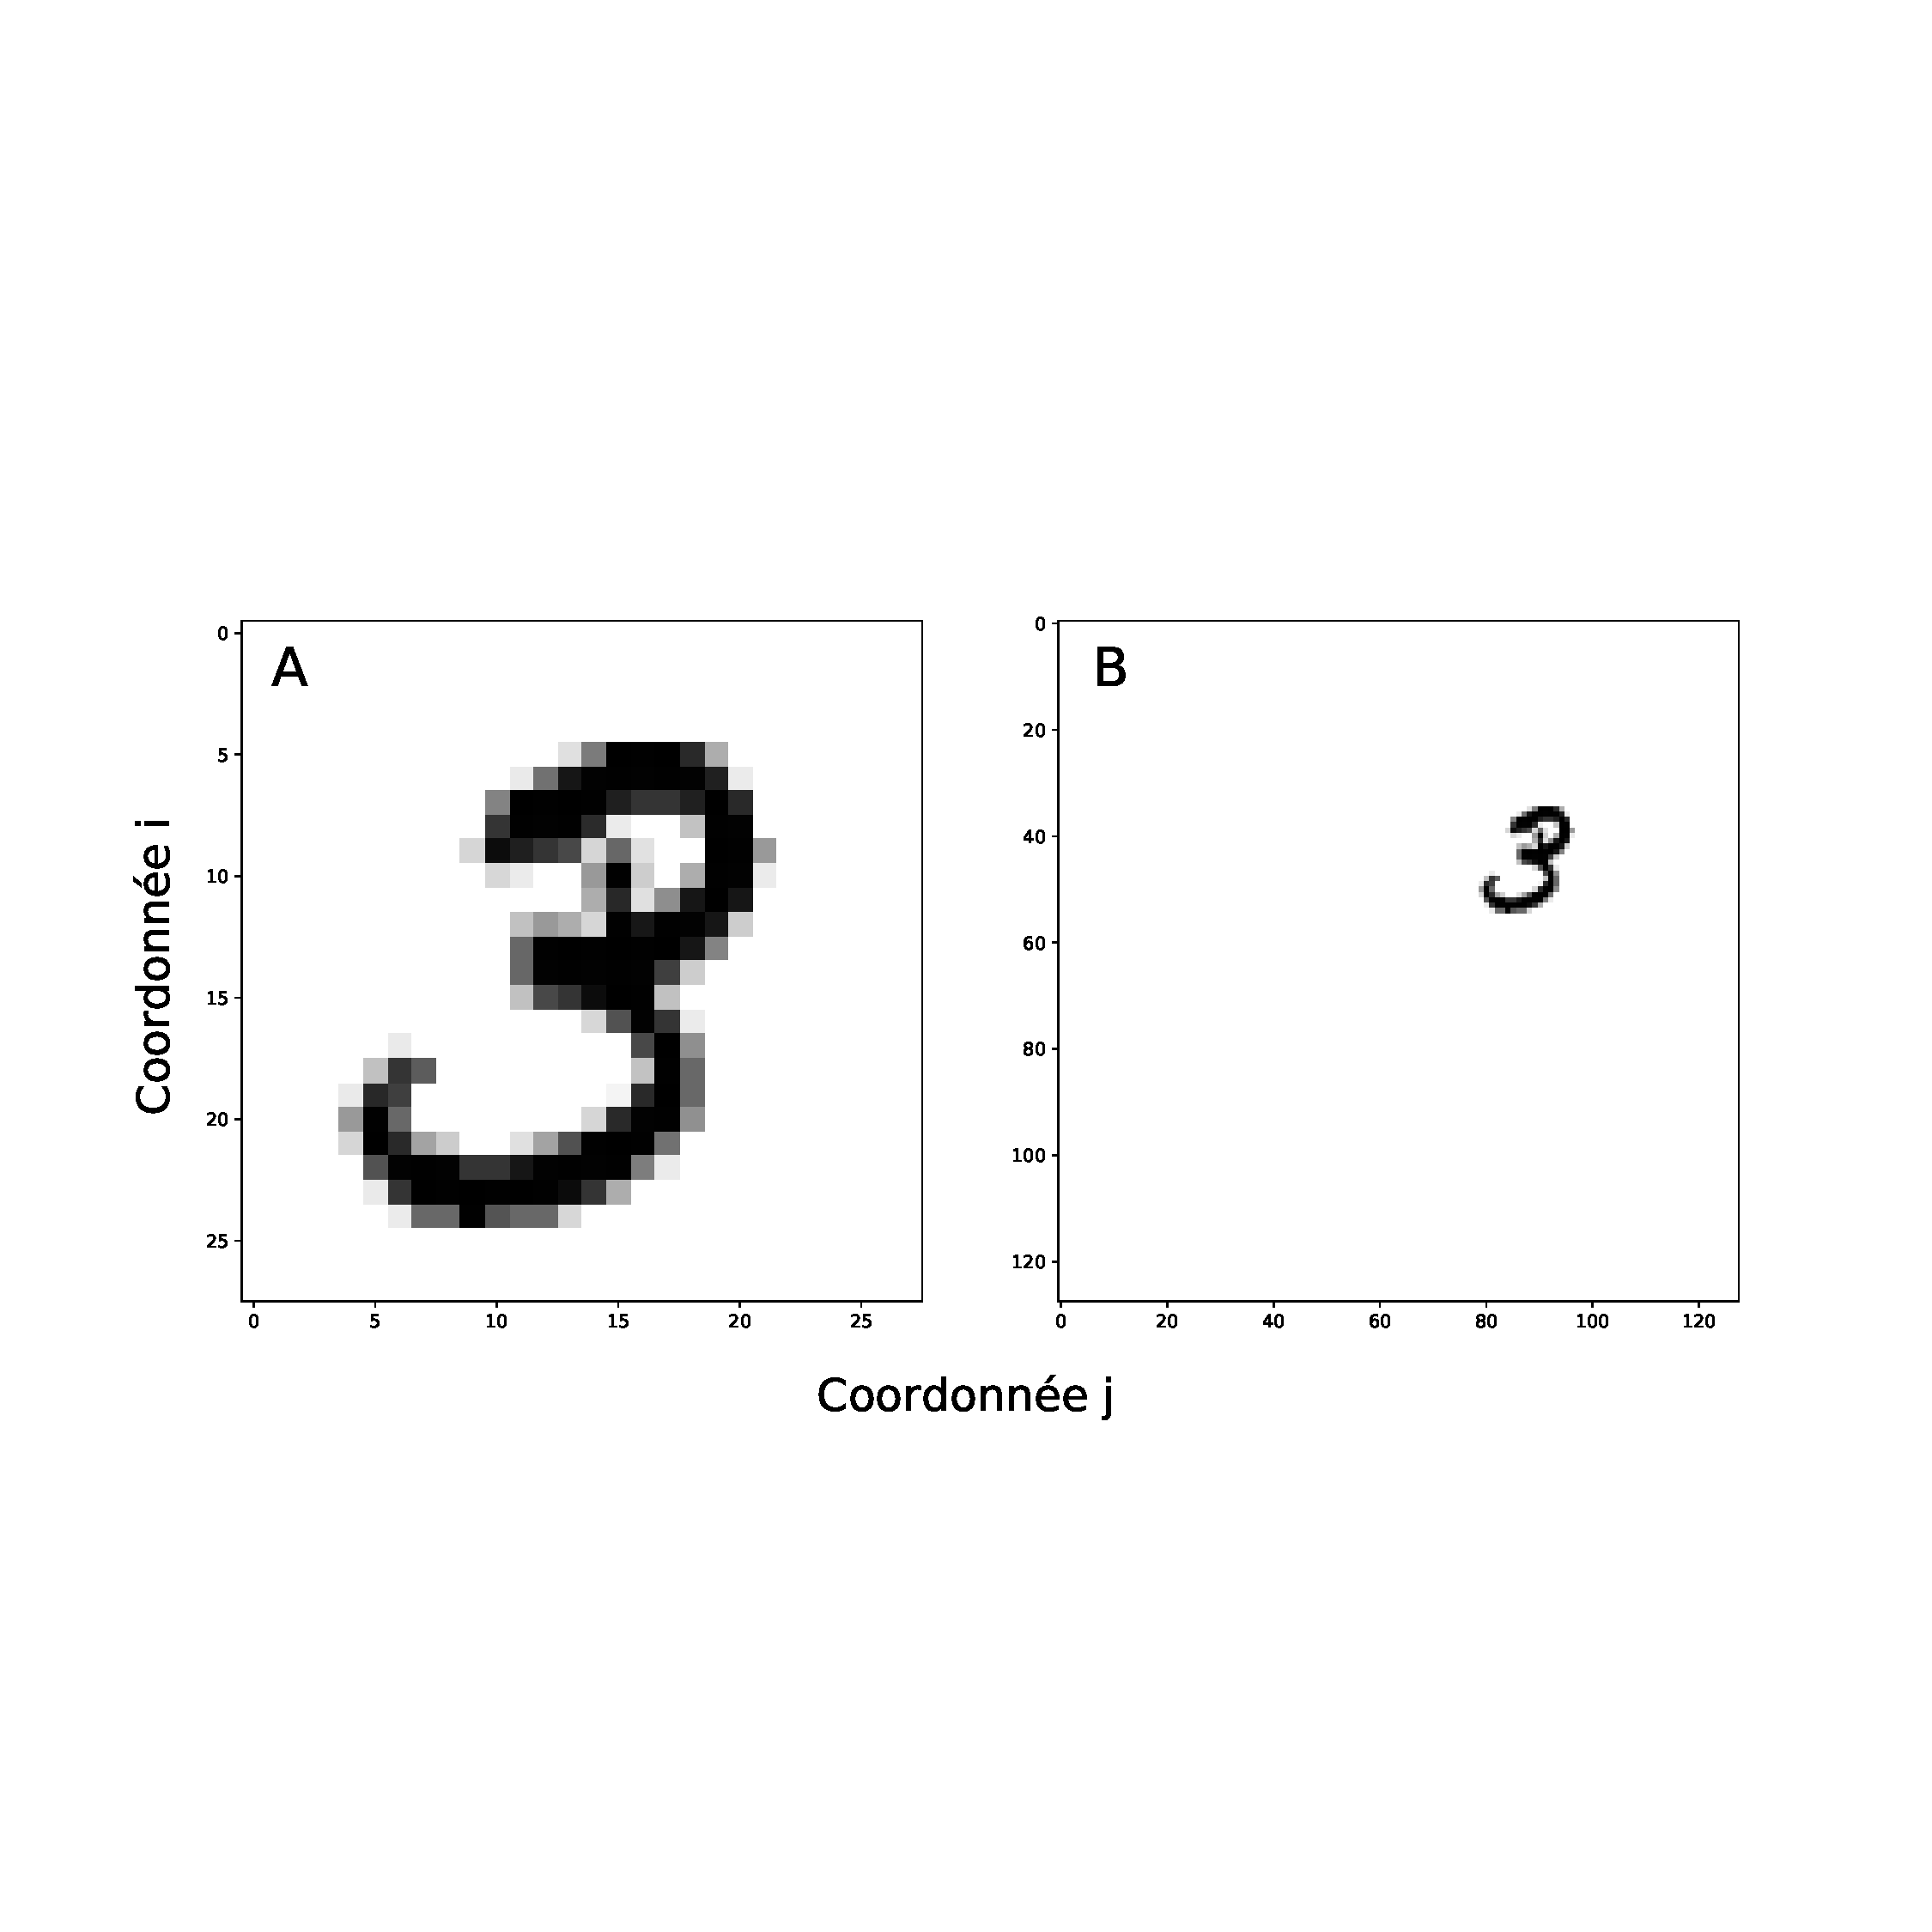
\includegraphics[scale=0.3]{Figures/mnist_reshape}
\decoRule %puts an aesthetic horizontal line below the image
\caption[Figure]{\textbf{A.} Image originale tirée de MNIST ; \textbf{B.} Image après transformation géométrique et placé aux coordonnées $(i=-20,j=25)$}
\label{fig:mnist_reshape}
\end{figure}

\begin{figure}[th]
\centering
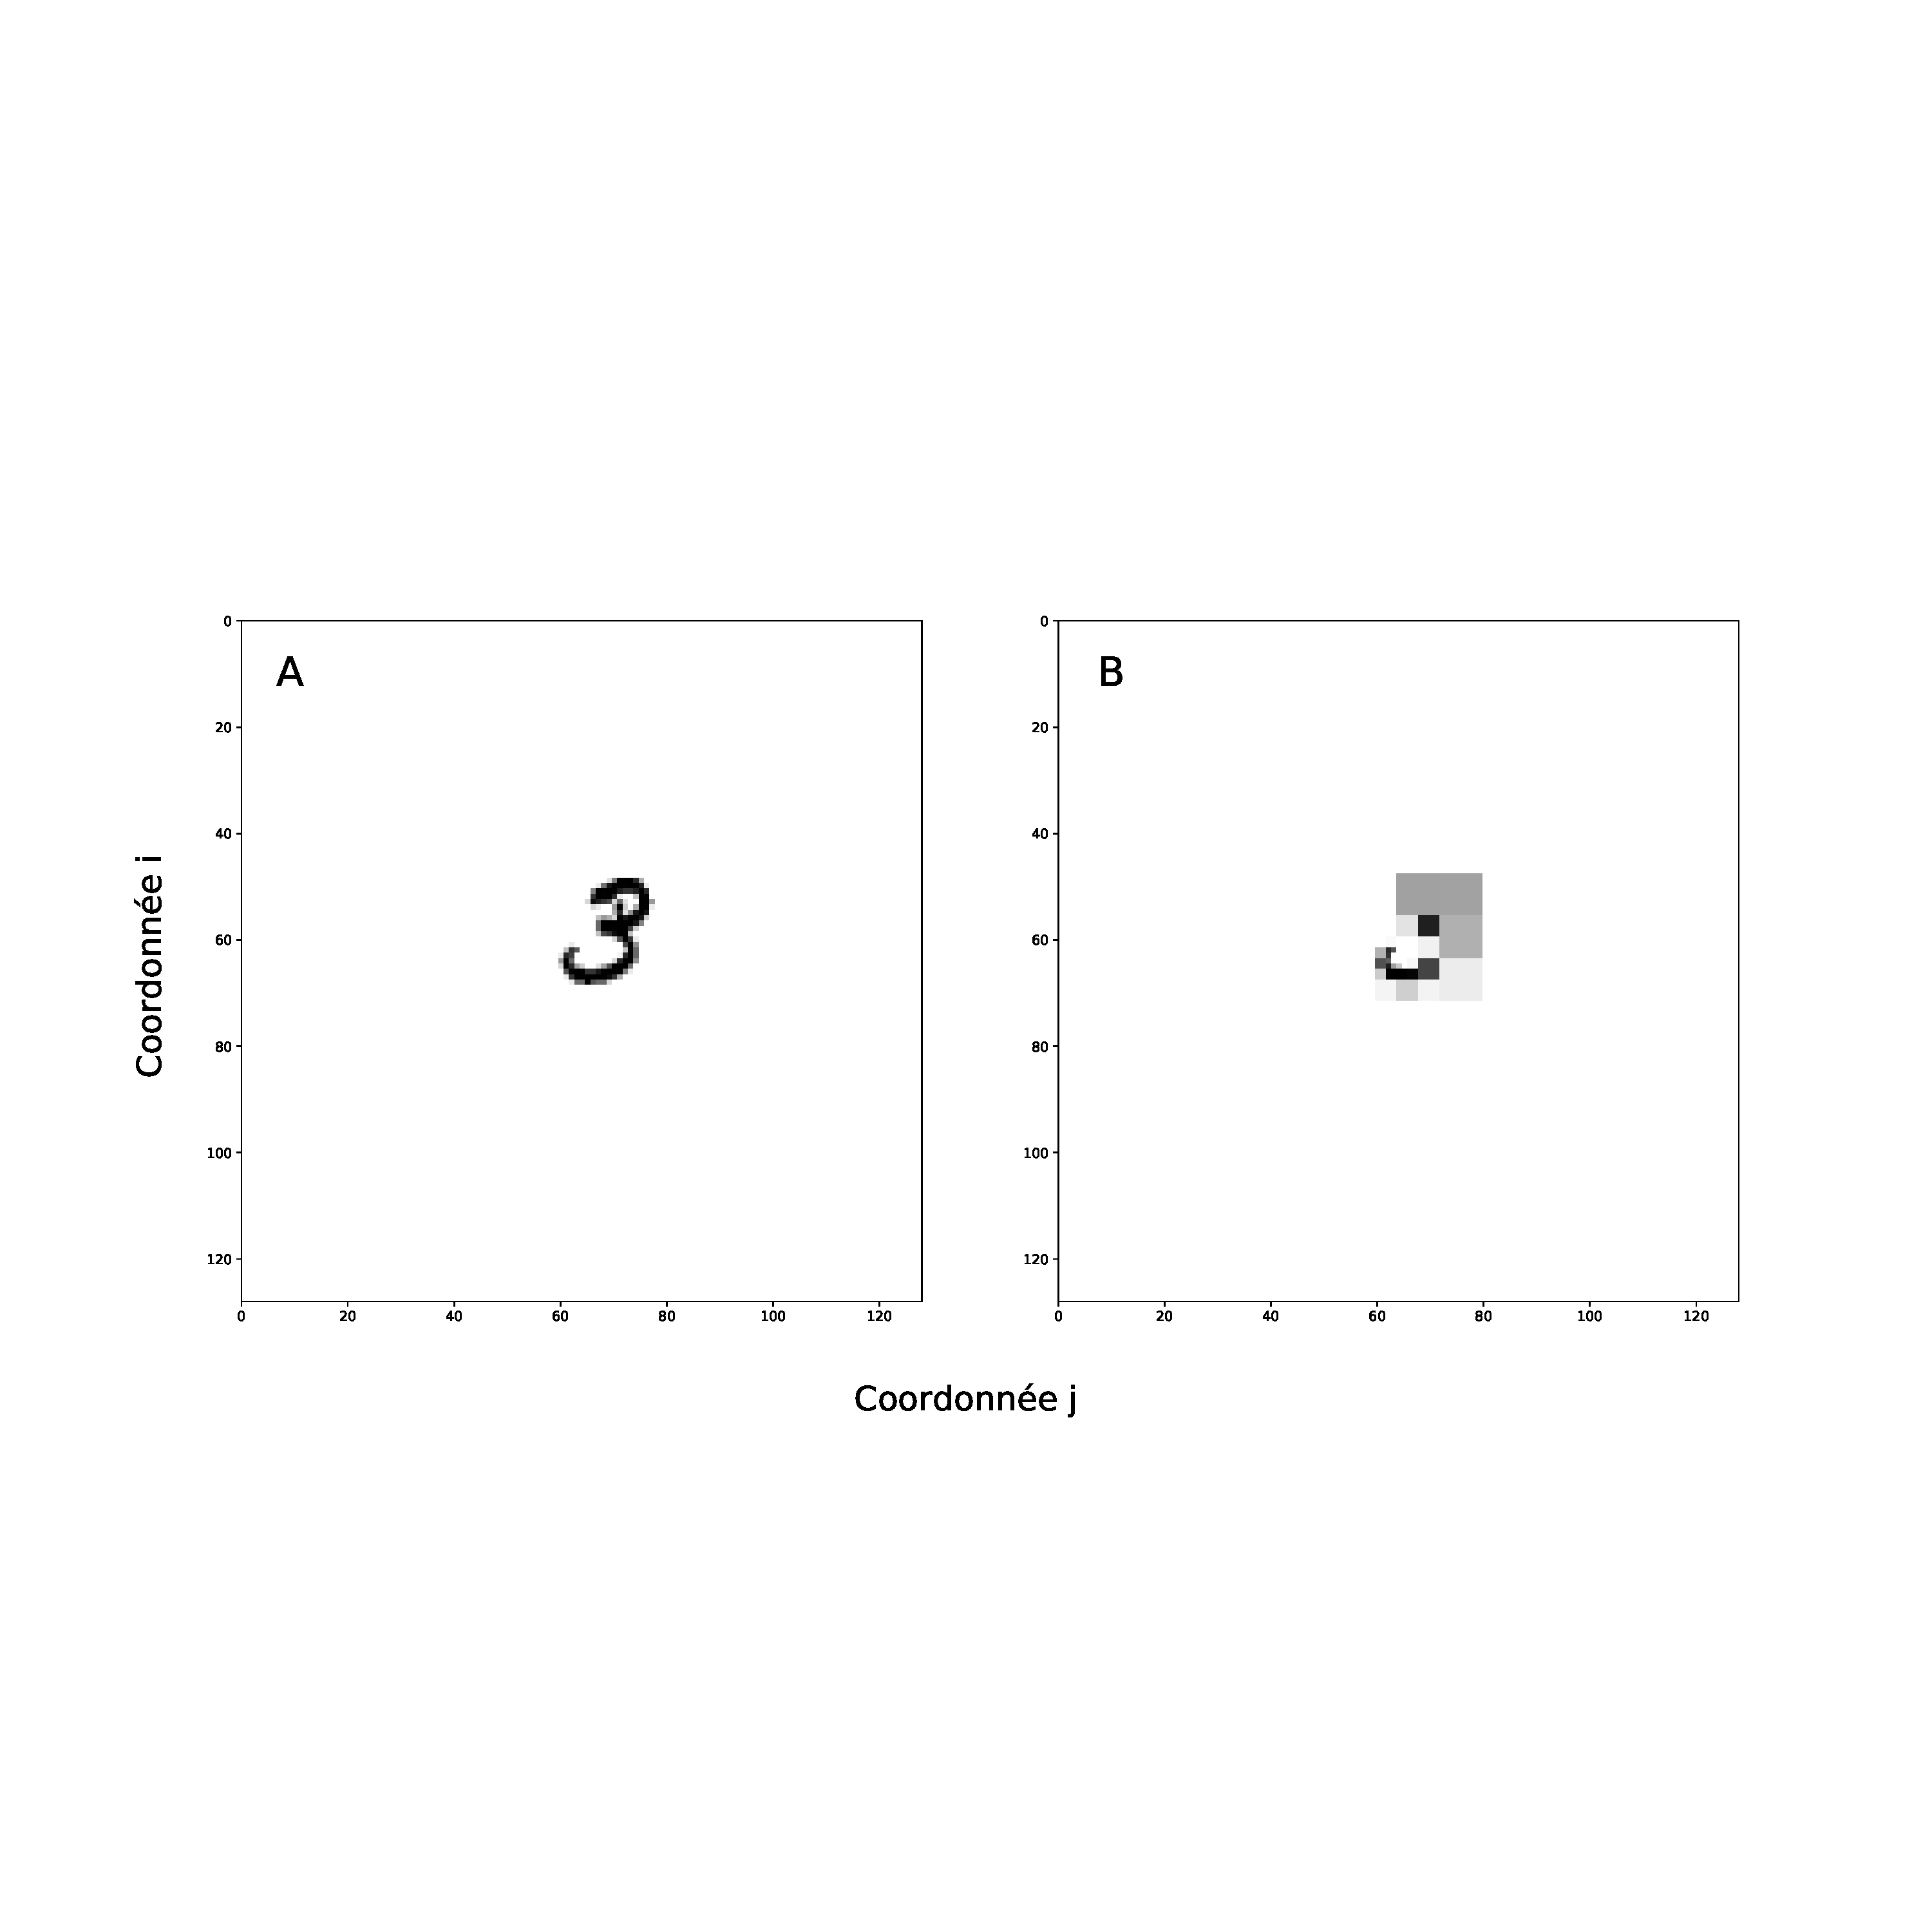
\includegraphics[scale=0.25]{Figures/wavelet_effect}
\decoRule %puts an aesthetic horizontal line below the image
\caption[Figure]{\textbf{A.} Image avant application d'un filtre et placé aux coordonnées $(i=-6,j=6)$ ; \textbf{B.} Image après transformation par le filtre \textit{Wavelets}}
\label{fig:Wavelet_effect}
\end{figure}

\begin{figure}[th]
\centering
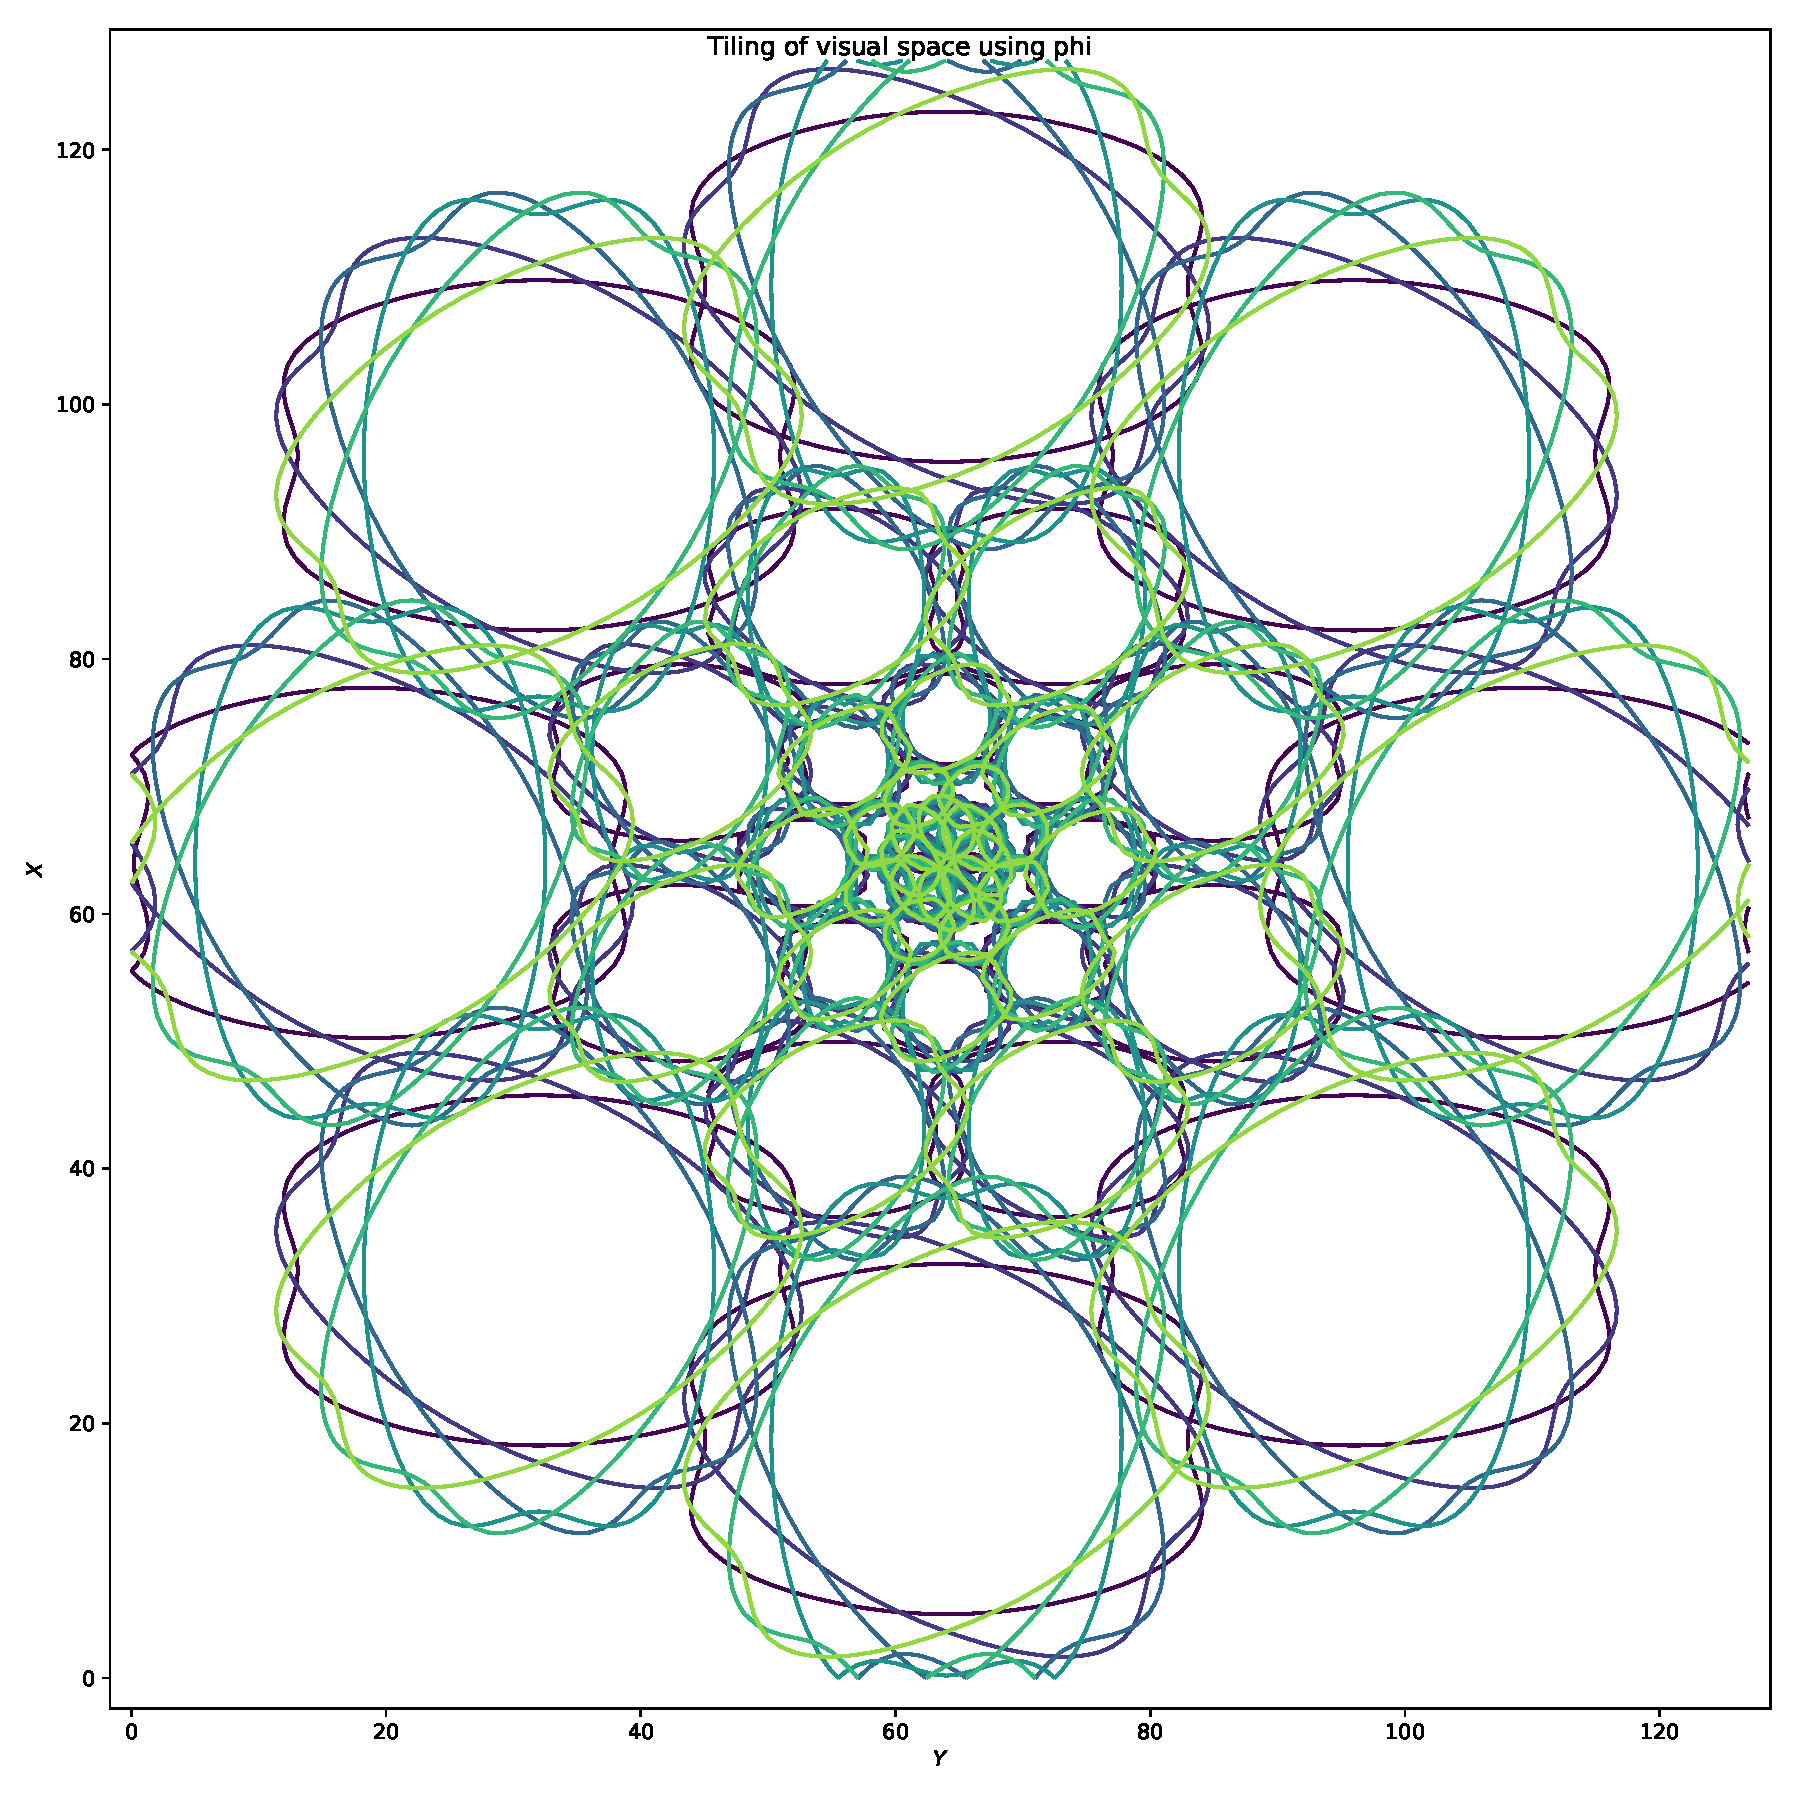
\includegraphics[scale=0.35]{Figures/LogPolar_shape}
\decoRule %puts an aesthetic horizontal line below the image
\caption[Figure]{Représentation graphique du filtre \textit{LogPolar} ($N_{theta}=6$,$N_{orient}=8$,$N_{scale}=5$,$N_{phase}=2$) }
\label{fig:LogPolar_shape}
\end{figure}

\begin{figure}[th]
\centering
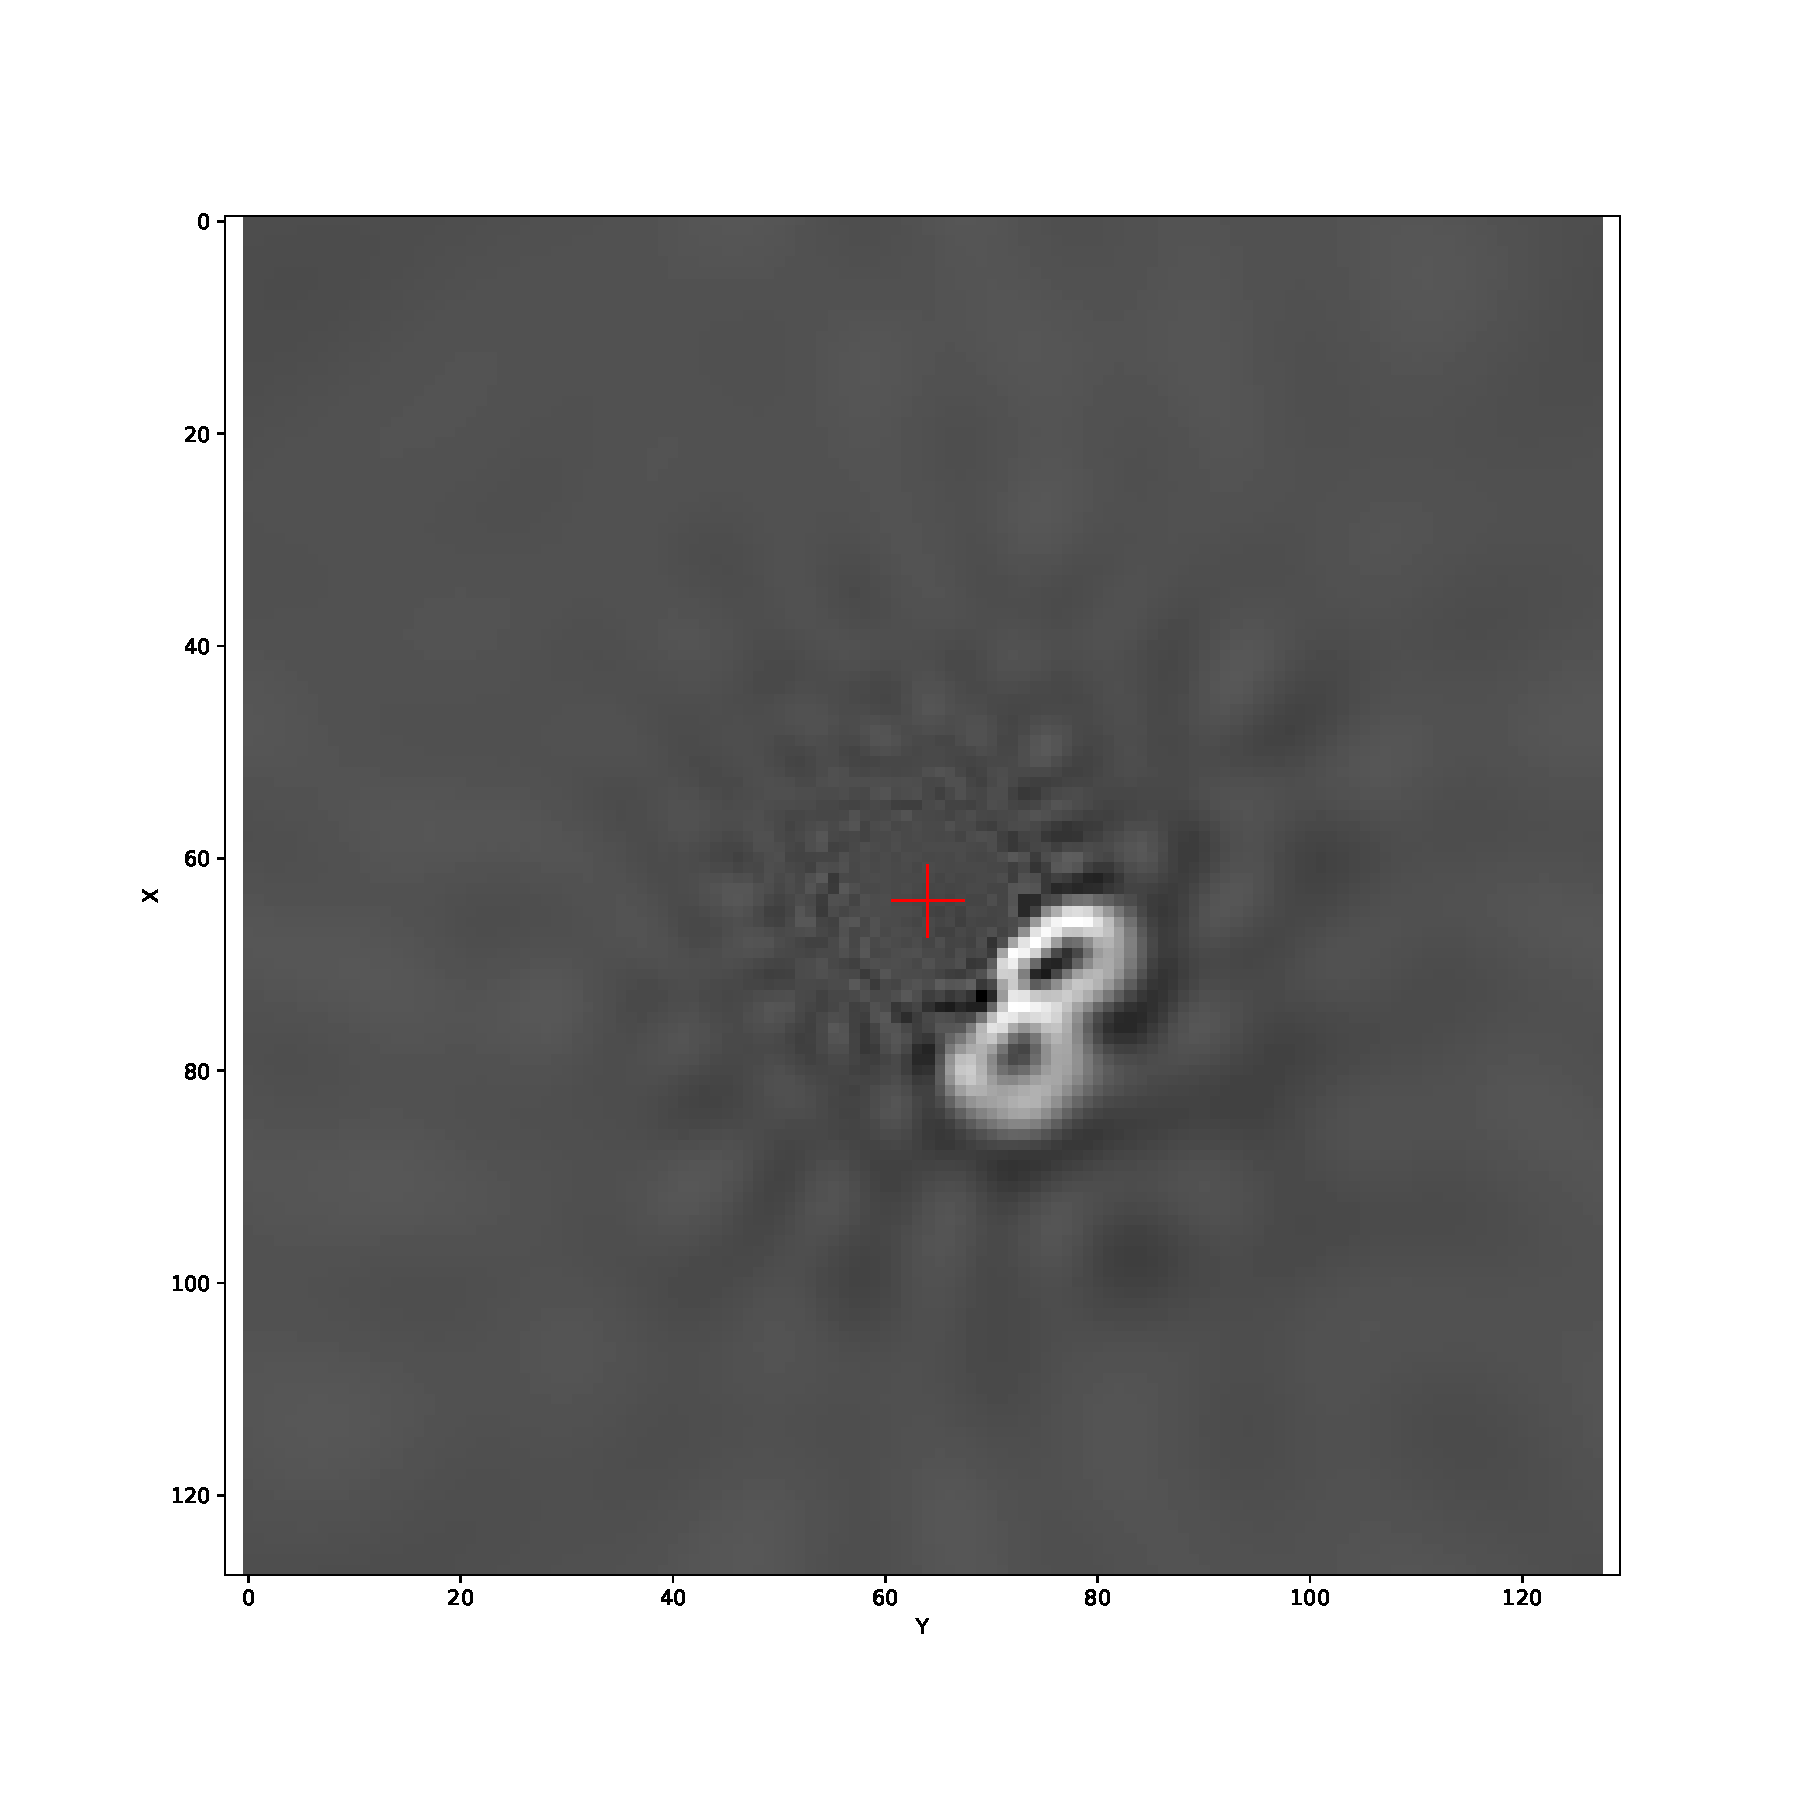
\includegraphics[scale=0.35]{Figures/LogPolar_effect}
\decoRule %puts an aesthetic horizontal line below the image
\caption[Figure]{Image après transformation par le filtre \textit{LogPolar} ($N_{theta}=6$,$N_{orient}=8$,$N_{scale}=5$,$N_{phase}=2$) }
\label{fig:LogPolar_effect}
\end{figure}

%%%%% Résultats %%%%%

\begin{figure}[th]
\centering
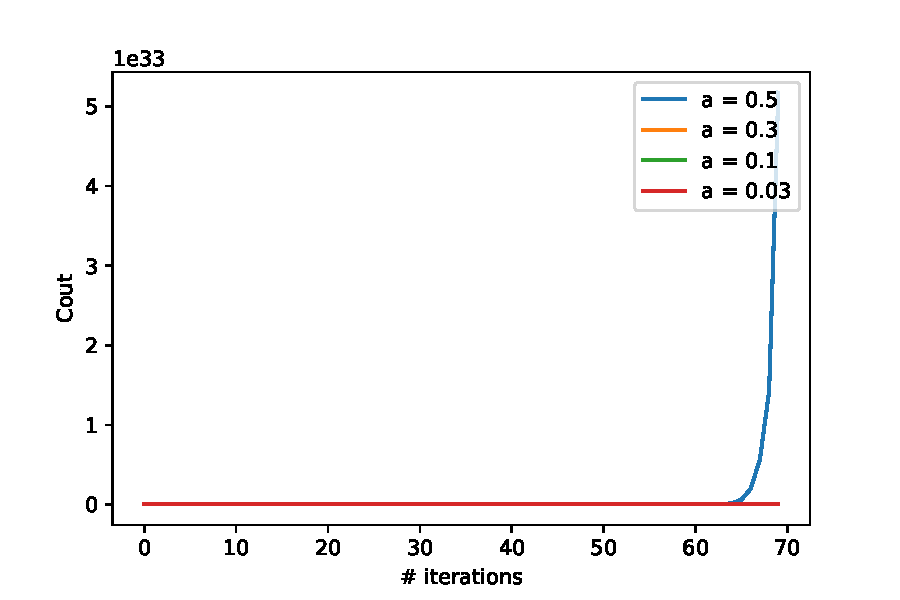
\includegraphics{Figures/Benchmarking_para_alpha_2}
\decoRule %puts an aesthetic horizontal line below the image
\caption[Figure]{Effet du paramètre alpha sur l'apprentissage dans le cadre d'un filtre \textit{Wavelets}}
\label{fig:benchmark_surApp1}
\end{figure}

\begin{figure}[th]
\centering
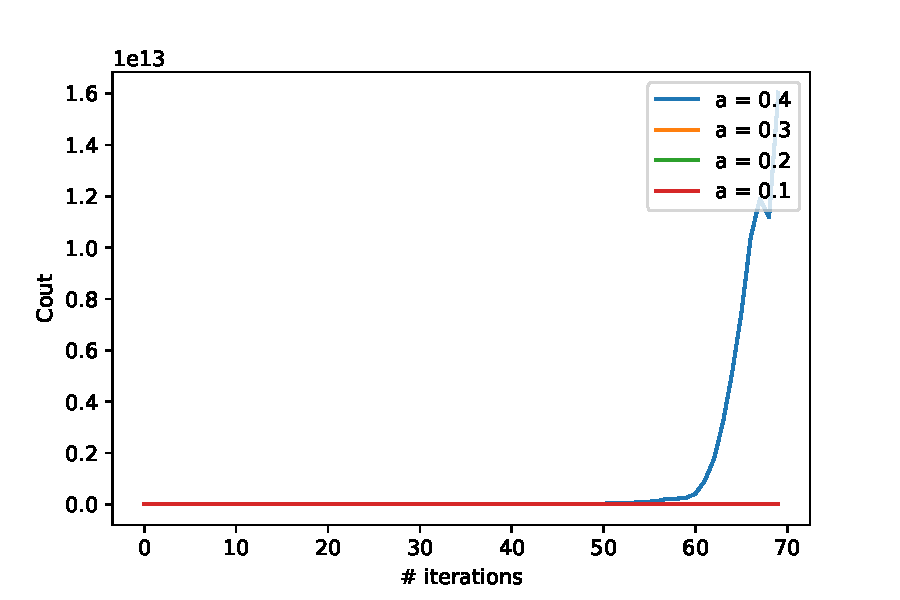
\includegraphics{Figures/Benchmarking_para_alpha_3}
\decoRule %puts an aesthetic horizontal line below the image
\caption[Figure]{Effet du paramètre alpha sur l'apprentissage dans le cadre d'un filtre \textit{Wavelets}}
\label{fig:benchmark_surApp2}
\end{figure}

\begin{figure}[th]
\centering
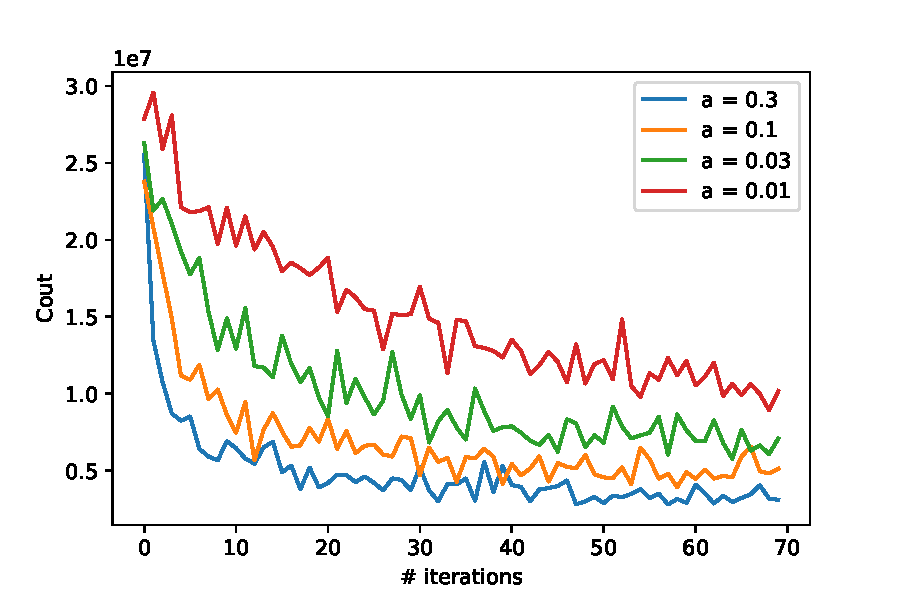
\includegraphics{Figures/Benchmarking_para_alpha}
\decoRule %puts an aesthetic horizontal line below the image
\caption[Figure]{Effet du paramètre alpha sur l'apprentissage dans le cadre d'un filtre \textit{Wavelets}}
\label{fig:benchmark_alpha}
\end{figure}

\begin{figure}[th]
\centering
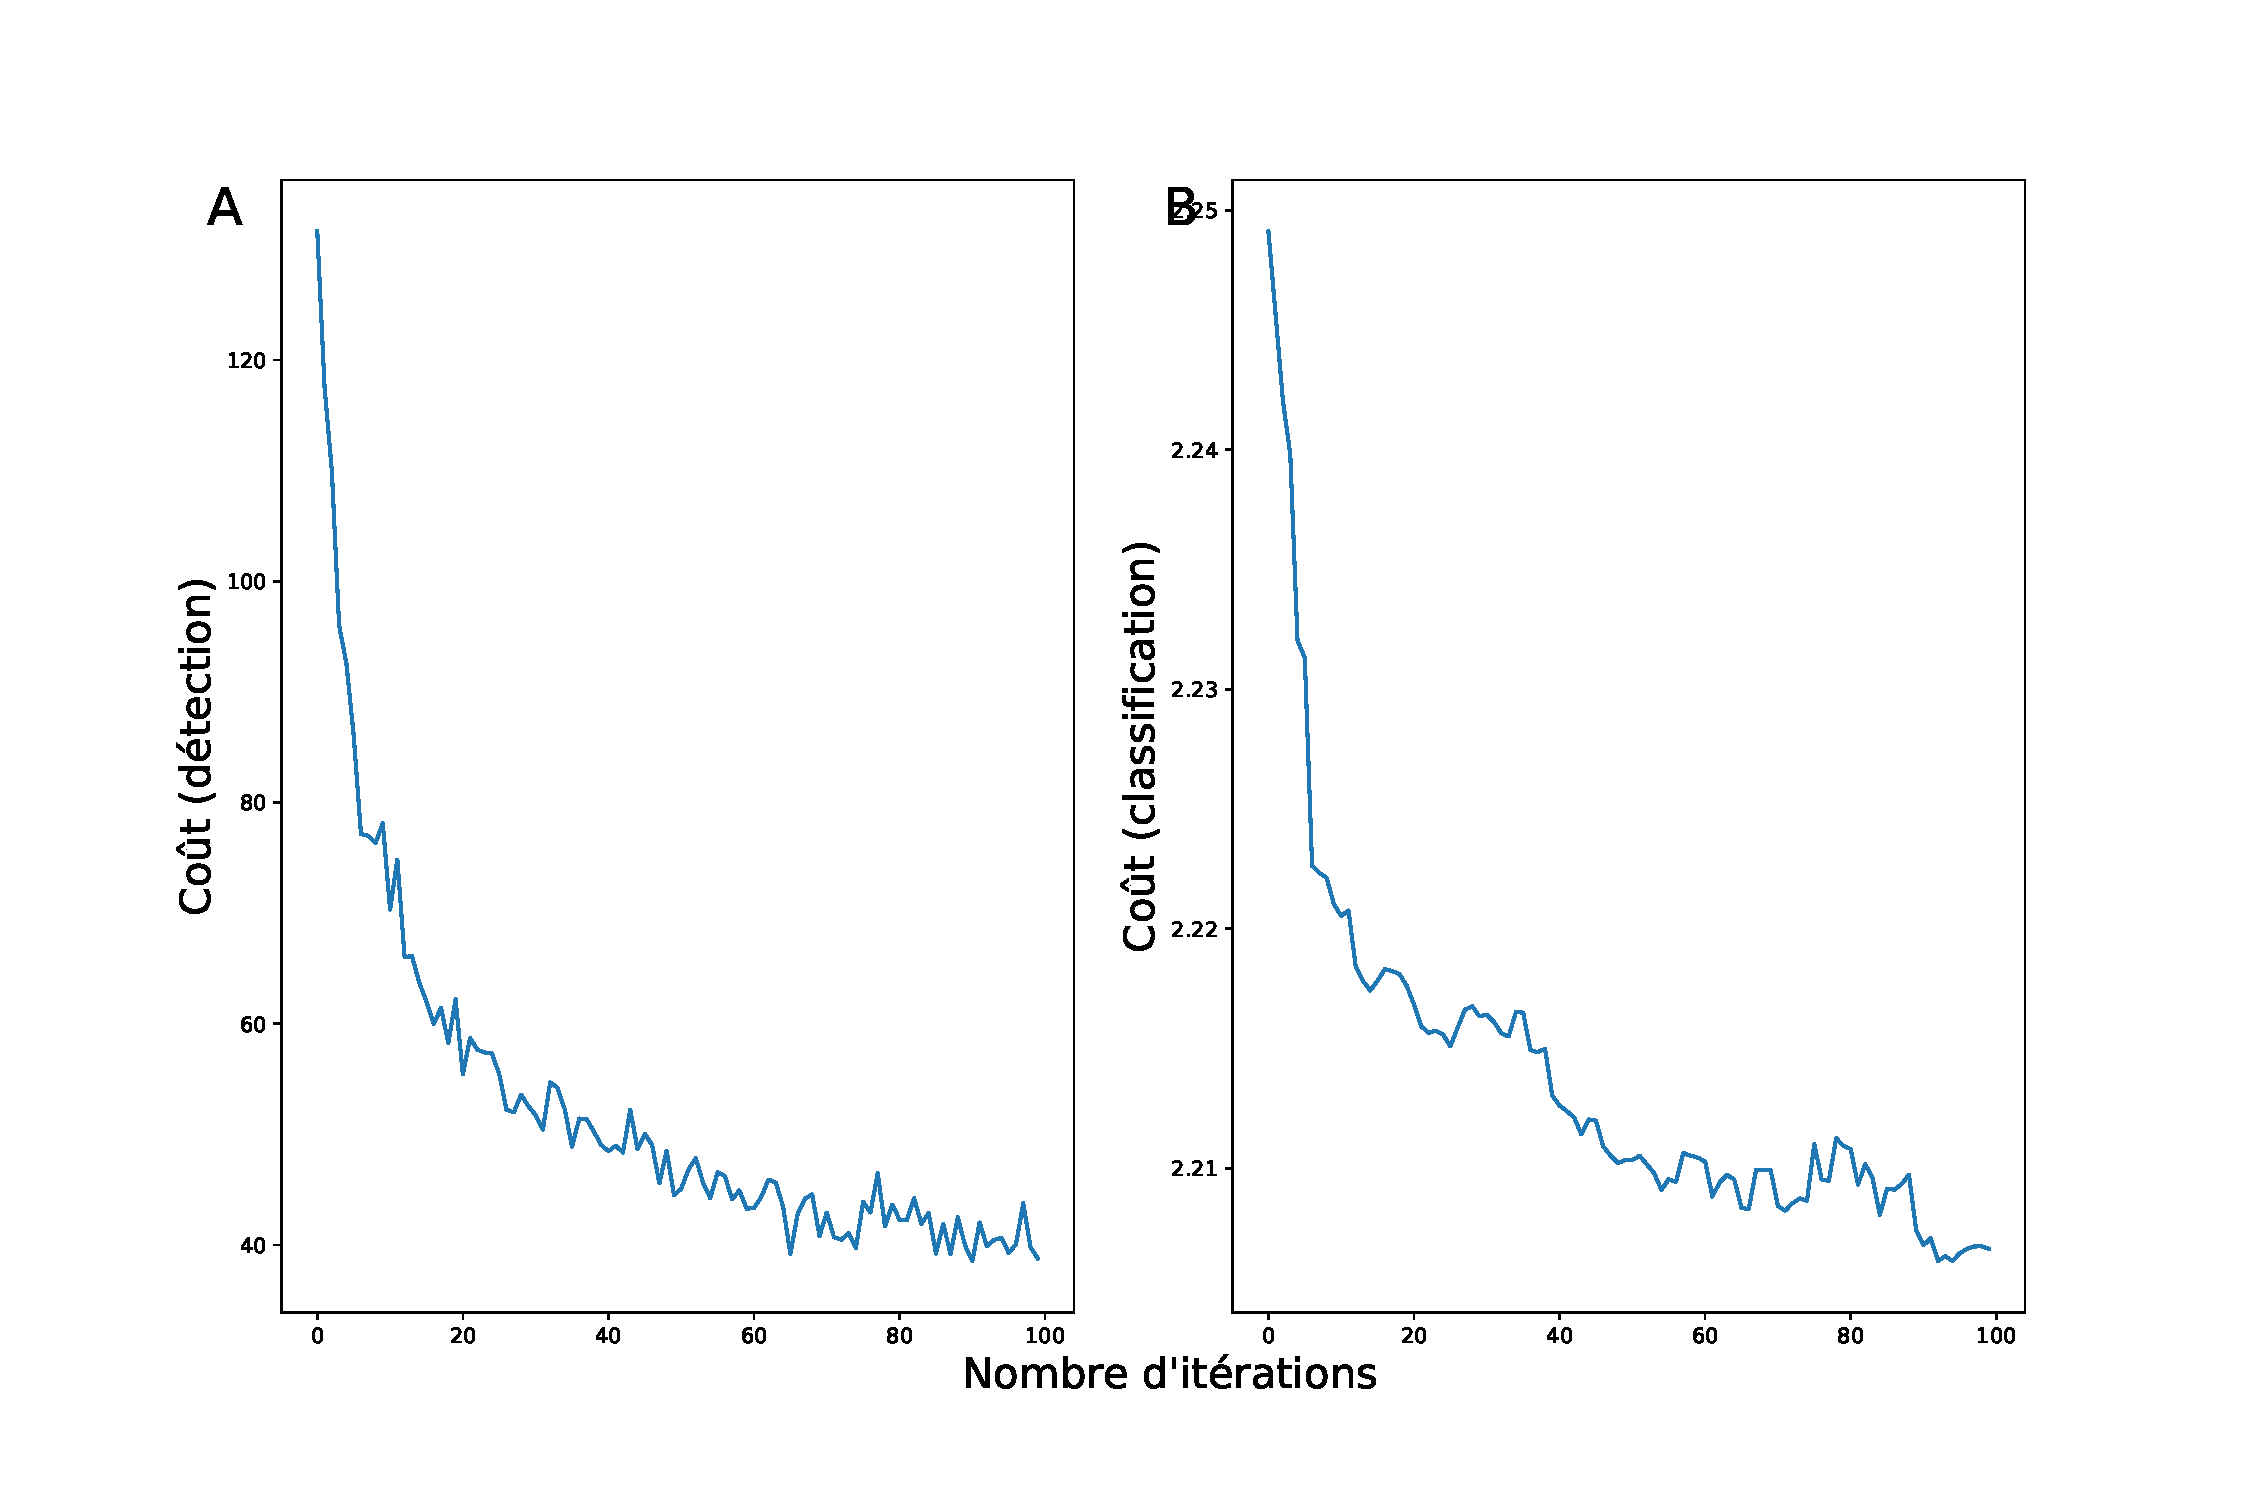
\includegraphics[scale=0.4]{Figures/logpolar_cost_learning}
\decoRule %puts an aesthetic horizontal line below the image
\caption[Figure]{Réduction du coût des couches \textit{détecteur} et \textit{classifieur} lors de l'apprentissage, dans le cadre d'un filtre \textit{LogPolar} (taille de la base d'apprentissage :  1000, nombre d'itérations : 100, $\alpha_{detect}=0.0015$, $\alpha_{classif}=0.3$)}
\label{fig:logpolar_cost}
\end{figure}

\begin{figure}[th]
\centering
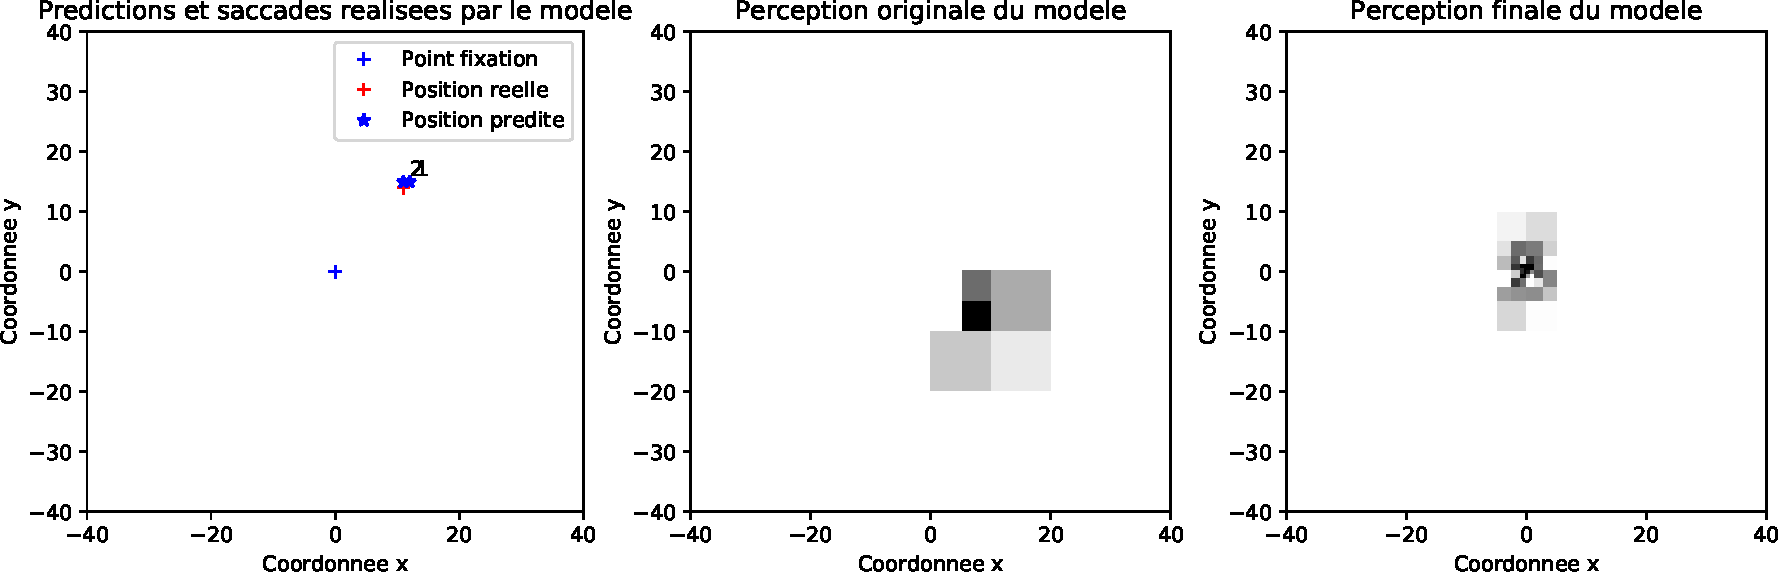
\includegraphics[scale=0.5]{Figures/saccades}
\decoRule %puts an aesthetic horizontal line below the image
\caption[Figure]{Perception et comportement saccadique du modèle entraîné, dans le cadre d'un filtre \textit{Wavelets}}
\label{fig:saccades}
\end{figure}

\begin{figure}[th]
\centering
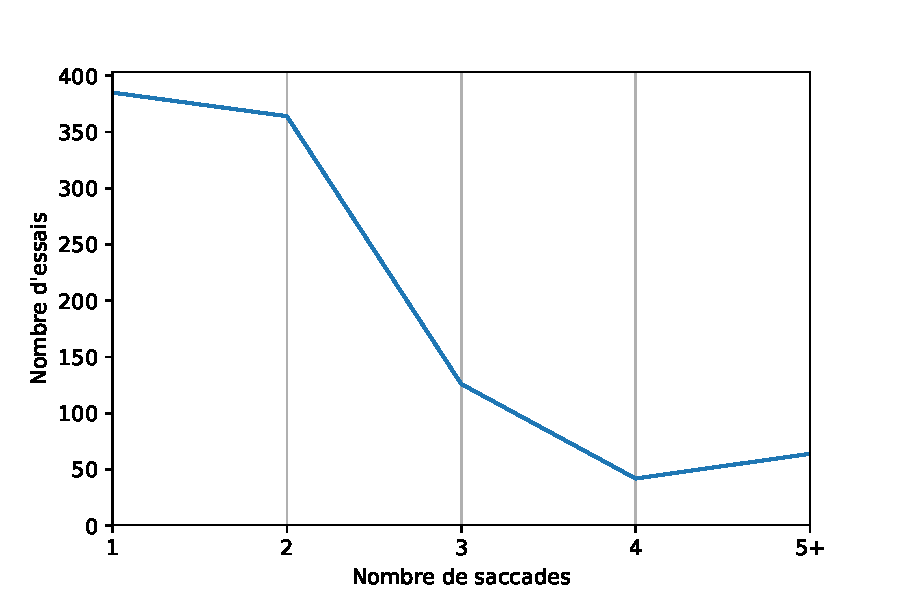
\includegraphics{Figures/sacc_nombre}
\decoRule %puts an aesthetic horizontal line below the image
\caption[Figure]{Nombre de saccades nécessaires pour atteindre la position de la cible au cours de 1000 essais, dans le cadre d'un filtre \textit{LogPolar} (taille de la base d'apprentissage :  1000, nombre d'itérations : 100, $\alpha_{detect}=0.0015$, $\alpha_{classif}=0.3$)}
\label{fig:sacc_nombre}
\end{figure}

\begin{figure}[th]
\centering
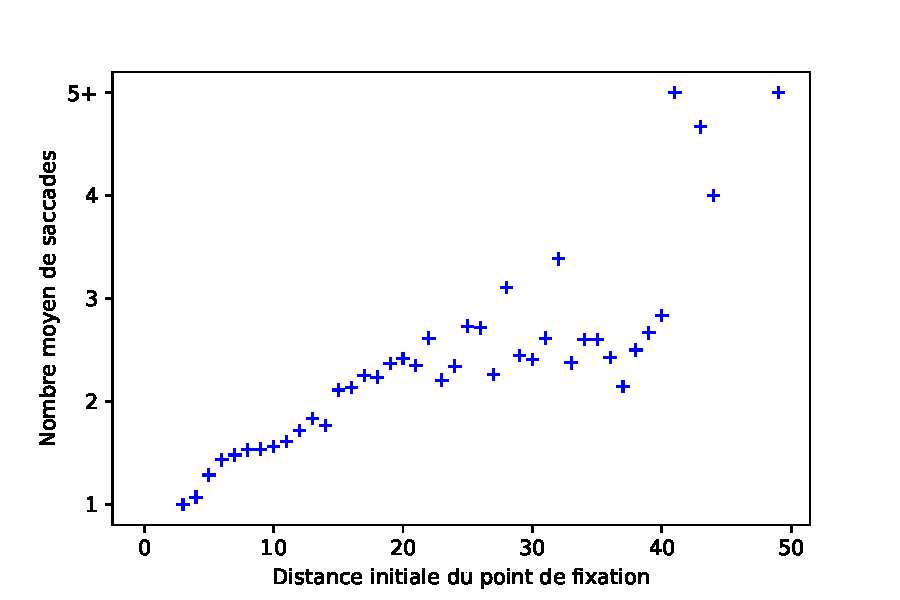
\includegraphics{Figures/sacc_distance}
\decoRule %puts an aesthetic horizontal line below the image
\caption[Figure]{Nombre moyen de saccades nécessaires pour atteindre la position de la cible en fonction de sa distance initiale du point de fixation au cours de 1000 essais, dans le cadre d'un filtre \textit{LogPolar} (taille de la base d'apprentissage :  1000, nombre d'itérations : 100, $\alpha_{detect}=0.0015$, $\alpha_{classif}=0.3$)}
\label{fig:sacc_distance}
\end{figure}

\begin{figure}[th]
\centering
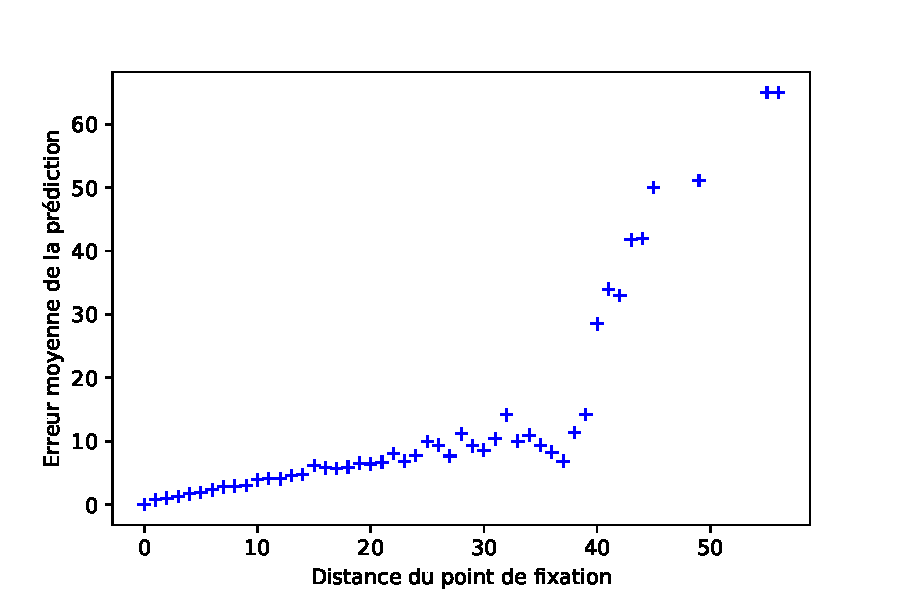
\includegraphics[scale=0.95]{Figures/err_distance}
\decoRule %puts an aesthetic horizontal line below the image
\caption[Figure]{Erreur moyenne lors de la prédiction de la position de la cible en fonction de sa distance du point de fixation au cours de 1000 essais, dans le cadre d'un filtre \textit{LogPolar} (taille de la base d'apprentissage :  1000, nombre d'itérations : 100, $\alpha_{detect}=0.0015$, $\alpha_{classif}=0.3$)}
\label{fig:err_distance}
\end{figure}
% Appendix Template

\chapter{Code source et documents complémentaires} % Main appendix title

\label{Code} % Change X to a consecutive letter; for referencing this appendix elsewhere, use \ref{AppendixX}

L'ensemble du code source du modèle sous forme de notebooks jupyter et de scripts python, de ce rapport au format \LaTeX~ainsi que de l'ensemble des autres documents issus de ce travail (dont les notes personnelles au format Markdown) sont entièrement disponibles \href{https://github.com/pierrealbiges/ActiveVision}{en ligne} ou en contactant directement l'\href{pierre.albiges@etu.univ-amu.fr}{auteur}.
%\include{Appendices/AppendixC}

%----------------------------------------------------------------------------------------
\end{document}  
